\documentclass[12pt,a4paper]{ctexart}
\usepackage[margin=2.6cm]{geometry}
\usepackage{amsmath,amssymb}
\usepackage{graphicx}
\usepackage{booktabs}
\usepackage{array}
\usepackage{longtable}
\usepackage{caption}
\usepackage{enumitem}
\pagestyle{plain}
\usepackage{fancyvrb}
\usepackage{xcolor}
\usepackage{hyperref}
\hypersetup{colorlinks=true,linkcolor=blue,urlcolor=blue}
\setcounter{tocdepth}{3}
\graphicspath{{figures/}{./}}
\setlength{\parindent}{2em}
\linespread{1.25}
% 等宽字体含制表符/箭头(Consolas)，中文等宽回退(宋体)，供 ASCII 框图使用
\IfFontExistsTF{DejaVu Sans Mono}{\setmonofont{DejaVu Sans Mono}[Scale=0.9]}{\IfFontExistsTF{Consolas}{\setmonofont{Consolas}}{}}
\IfFontExistsTF{SimSun}{\setCJKmonofont{SimSun}}{}
\fvset{fontsize=\footnotesize,frame=single,framesep=4pt}
\title{\bfseries 面向雷达情报的可解释知识图谱问答与对抗决策支持方法研究}
\author{}
\date{}
\begin{document}
\maketitle
\tableofcontents
\newpage


\subsection*{摘要}
\addcontentsline{toc}{subsection}{摘要}

随着现代战场电磁环境日趋复杂，雷达情报的规模、异构性与时效性持续增长，如何对海量雷达装备知识进行有效组织、可靠问答与进一步的对抗决策辅助，已成为军事智能化的重要课题。近年来，大语言模型（Large Language Model, LLM）与知识图谱（Knowledge Graph, KG）相结合的检索增强生成（Retrieval-Augmented Generation, RAG）方法在开放域问答中取得显著进展，但直接迁移到雷达情报这一\textbf{专业性强、可解释性要求高、且最终服务于决策}的领域时，仍面临三方面困难：其一，通用 GraphRAG 对不同"问题形态"缺乏针对性，检索召回与问题所需的图结构不匹配；其二，生成式模型存在幻觉，难以满足情报分析对结论可溯源、可审计的刚性要求；其三，从"知道是什么"到"建议怎么办"的对抗决策，需要将稀疏且异构的电子战学理知识形式化，而现有方法多为面向特定干扰样式的强化学习黑箱，缺乏可解释性与知识可溯源性。

针对上述问题，本文以雷达情报领域为背景，构建了一条"\textbf{构建知识图谱 → 可解释问答 → 可审计分析 → 对抗决策支持}"的递进式技术路线，主要工作与创新点如下：

\textbf{（1）雷达领域可溯源知识图谱构建。} 设计了面向雷达装备的属性图模式，融合领域手册、百科与开放知识库进行多源抽取，为每条事实附加来源、置信度与证据元数据，形成规模达万级三元组、支持可溯源查询的领域知识图谱，为后续问答与决策提供统一知识底座。

\textbf{（2）策略路由的 GraphRAG 与"答案-几何失配"诊断。} 提出并形式化了"答案-几何失配"（Answer-Geometry Mismatch, AGM）现象，揭示通用 GraphRAG 在不同问题形态上失效的结构性根因；据此设计 O(1) 复杂度的问题分发器与六类\textbf{类型化检索算子}，使检索结构与问题所需几何相匹配。在自建的、显式暴露该失配的领域基准 RadarKG-QA-499 上，方法取得 88.6\% 的总体准确率，较 Top-K 基线提升 35.9 个百分点、较 RoG 提升 28.3 个百分点；消融实验表明增益由算子设计驱动（分发器贡献约 0 个百分点）。

\textbf{（3）双层可审计分析智能体。} 将单次问答升级为"内层类型化算子组合执行器 + 外层 ReAct 编排"的双层智能体，并提出"大语言模型不进入信任路径"的可审计架构原则：关键事实与数字由确定性执行轨迹生成，模型仅承担受约束的自然语言复述。算子组合评测正确率 99\%，情报报告逐条引证覆盖率与概述可溯源率均达 100\%。

\textbf{（4）面向雷达对抗的可解释决策支持。} 将电子战对抗学理形式化为知识图谱上的推理：以反制关系刻画干扰与抗干扰的博弈，给出"可行/被抵消/应避免"三分输出的确定性推理算子并证明其可审计性；将战场级对抗方案归约为加权集合覆盖问题，给出具有 $H_n$ 近似保证的贪心算法；构建覆盖九个国家、三十余个防空体系、八十余部威胁雷达的可溯源威胁库与对抗本体，并以已解密战史作为独立检验。教科书级对抗案例测试通过率 100\%，全部画像满足引擎不变量。

\textbf{（5）面向自适应雷达的知识引导在线对抗学习。} 针对认知电子战中威胁雷达\textbf{反应式切换抗干扰}这一序贯、部分可观测特性，将对抗手段选择形式化为隐藏抗干扰(ECCM)状态下的在线学习问题，提出以 doctrine 反制图为\textbf{结构先验}的贝叶斯学习算法——经由每轮干扰成败沿反制关系反推雷达隐藏的抗干扰，其样本复杂度与抗干扰数相关而\textbf{与候选手段数无关}；并以变点检测应对雷达变招、以第三章主雷达图谱属性提供逐雷达先验，使知识图谱由"被查询"升级为"驱动学习"。在合成、\textbf{真实 doctrine 图}与\textbf{真实威胁雷达属性}上的仿真表明，该学习器稳定优于静态学理与强知识盲在线学习基线；本文并诚实界定其相对静态策略的密度-时长适用边界，以及"知识真实、对抗动态为仿真、效能非实测"的性质。

本文工作贯穿"\textbf{类型化算子}"与"\textbf{可解释、可溯源、不确定性显式建模}"两条主线，验证了在专业性强、知识稀疏、决策代价高的领域中，构造结论可审计、不确定性可传播、并具理论保证的智能分析与决策支持系统的可行性。

\textbf{关键词：} 知识图谱；检索增强生成；大语言模型；可解释问答；电子战；雷达对抗决策；集合覆盖


\subsection*{Abstract}
\addcontentsline{toc}{subsection}{Abstract}

As the electromagnetic battlespace grows increasingly complex, the scale, heterogeneity, and timeliness of radar intelligence continue to rise, making the effective organization, reliable question answering, and downstream countermeasure decision support over massive radar knowledge a key topic in military intelligentization. Recently, Retrieval-Augmented Generation (RAG) methods that combine Large Language Models (LLMs) with Knowledge Graphs (KGs) have achieved notable progress in open-domain question answering. However, transferring them directly to radar intelligence—a domain that is highly specialized, demands strong explainability, and ultimately serves decision-making—still faces three difficulties: (i) generic GraphRAG is not tailored to different "question shapes," so retrieval recall mismatches the graph structure a question actually requires; (ii) generative models hallucinate, failing the rigid requirement of traceable and auditable conclusions in intelligence analysis; and (iii) moving from "knowing what" to "advising what to do" requires formalizing sparse, heterogeneous electronic-warfare doctrine, whereas existing methods are mostly reinforcement-learning black boxes targeting specific jamming patterns, lacking explainability and provenance.

To address these problems, this thesis develops, in the radar-intelligence domain, a progressive technical roadmap of "\textbf{building a knowledge graph → explainable question answering → auditable analysis → countermeasure decision support}." The main contributions are:

\textbf{(1) A provenance-aware radar-domain knowledge graph.} A property-graph schema for radar equipment is designed; multi-source extraction fuses domain handbooks, encyclopedias, and open knowledge bases, attaching source, confidence, and evidence metadata to each fact, yielding a domain KG of tens of thousands of triples that supports traceable queries.

\textbf{(2) Strategy-routed GraphRAG and the Answer-Geometry Mismatch (AGM) diagnosis.} We formalize the AGM phenomenon that explains the structural root cause of generic GraphRAG's failures across question shapes, and design an O(1) dispatcher with six typed retrieval operators that align retrieval structure with the geometry a question requires. On RadarKG-QA-499, a domain benchmark built to expose this mismatch, the method attains 88.6\% overall accuracy—35.9 points above the Top-K baseline and 28.3 points above RoG—with ablations showing the gain is operator-driven (the dispatcher contributes about 0 points).

\textbf{(3) A two-layer auditable analysis agent.} Single-shot QA is upgraded to a two-layer agent—an inner typed operator-composition executor plus an outer ReAct orchestrator—under the architectural principle that "the LLM does not enter the trust path": critical facts and numbers are produced by a deterministic execution trace, while the model only paraphrases under constraints. Operator composition reaches 99\% accuracy, with 100\% citation coverage and 100\% summary faithfulness in intelligence reports.

\textbf{(4) Explainable countermeasure decision support against radar.} EW doctrine is formalized as reasoning over a KG: a counter-relation models the jamming/anti-jamming game; a deterministic operator yields a three-way output (viable / neutralized / avoid) and is proven auditable; battlefield-level planning is reduced to weighted set cover with a greedy $H_n$-approximation algorithm. A provenance-aware threat library and doctrine ontology covering 80+ threat radars across 9 countries and 30+ air-defense systems are built and validated against declassified combat history. Textbook-level countermeasure cases pass at 100\%, and all profiles satisfy the engine invariants.

\textbf{(5) Knowledge-guided online countermeasure learning against adaptive radars.} Addressing the sequential, partially observed nature of cognitive EW—where a threat radar reactively switches its ECCM—countermeasure selection is formalized as online learning under a hidden ECCM state. We propose a Bayesian learner that uses the doctrine counter-relation graph as a structural prior: from each round's success/defeat it infers the radar's hidden ECCM along the counter-relations, achieving a sample complexity that depends on the number of ECCM but is independent of the number of candidate techniques. Change-point detection handles radar mode switching, and attributes from the main radar KG (Ch.3) provide a per-radar prior—turning the KG from something queried into something that drives learning. Simulations on synthetic, real-doctrine, and real-threat-attribute settings show the learner consistently beats both static doctrine and strong knowledge-blind online learners; the thesis also honestly delimits its density/horizon regime of advantage over the static policy and the "real knowledge, simulated dynamics, non-measured effectiveness" nature of the study.

This thesis is unified by two threads—\textbf{typed operators} and \textbf{explainable, traceable, uncertainty-aware reasoning}—demonstrating the feasibility of building auditable, theoretically grounded intelligent analysis and decision-support systems for specialized, knowledge-sparse, high-stakes domains.

\textbf{Keywords:} Knowledge Graph; Retrieval-Augmented Generation; Large Language Model; Explainable Question Answering; Electronic Warfare; Radar Countermeasure Decision; Set Cover



\section*{符号表与缩略语}
\addcontentsline{toc}{section}{符号表与缩略语}

\subsection*{主要符号}
\addcontentsline{toc}{subsection}{主要符号}

\begin{center}\small
\begin{tabular}{|p{0.307\textwidth}|p{0.307\textwidth}|p{0.307\textwidth}|}
\hline
\textbf{符号} & \textbf{含义} & \textbf{首次出现} \\ \hline
$G=(V,E,A,\ell,\mathrm{prov})$ & 属性图：实体、边、属性、类型标注、可溯源元数据 & §3.2 \\ \hline
$(h,r,t)$ & 三元组：头实体、关系、尾实体 & §2.1 \\ \hline
$\mathrm{prov}(x)=(\mathrm{source},\mathrm{conf},\mathrm{evidence})$ & 声明 $x$ 的来源/置信度/证据 & §3.4 \\ \hline
$I(q)$ & 问题 $q$ 的最小信息需求 & §4.2 \\ \hline
$K$ & Top-K 检索的截断常数 & §4.1 \\ \hline
$\mathcal{G}$ & 计划树文法（可嵌套算子代数） & §5.3 \\ \hline
$\mathrm{eval}(P)$ & 计划树 $P$ 的确定性求值（值 + 轨迹） & §5.3 \\ \hline
$\delta(P)$ & 由执行轨迹生成的权威答案 & §5.4 \\ \hline
$\psi$ & 大模型对权威答案的受约束自然语言复述 & §5.4 \\ \hline
$\pi(r)$ & 威胁雷达 $r$ 的威胁画像（属性上的部分函数） & §6.2 \\ \hline
$\mathcal{A}$ & 威胁画像属性集（用途/跟踪体制/频段/频率/功率/捷变…） & §6.2 \\ \hline
$J,\ E$ & 干扰技术集合、抗干扰（ECCM）技术集合 & §6.2 \\ \hline
$\mathcal{D}\subseteq E\times J$ & 反制关系：$(e,j)\in\mathcal{D}$ 表 $e$ 克制 $j$ & §6.2 \\ \hline
$\mathcal{P},\ \rho$ & 学理规则集；单条规则 $(\mathrm{cond}_\rho,\mathrm{rec}_\rho,\mathrm{avoid}_\rho,c_\rho,\mathrm{src}_\rho)$ & §6.2 \\ \hline
$F(r)$ & 对威胁 $r$ 点火的规则集 & §6.5 \\ \hline
$\widehat{R}(r),\ A(r),\ N(r)$ & 推荐集、避免集、被对方 ECCM 中和的集合 & §6.5 \\ \hline
$\mathrm{Viab}/\mathrm{Cnt}/\mathrm{Avoid}(r)$ & 三分输出：可行 / 被抵消 / 应避免 & §6.5 \\ \hline
$c(j\mid r)$ & 干扰技术 $j$ 对威胁 $r$ 的置信度 & §6.5 \\ \hline
$\Gamma(r)$ & 按本机定量参数生成的交战研判 & §6.5 \\ \hline
$\mathrm{cover}(s,r)$ & 装备 $s$ 可交战威胁 $r$ 的谓词 & §6.6 \\ \hline
$w(r)$ & 威胁 $r$ 的威胁度权重 & §6.6 \\ \hline
$H_n=\sum_{k=1}^n 1/k$ & 第 $n$ 调和数（集合覆盖近似比 $\le\ln n+1$） & §6.6 \\ \hline
\end{tabular}
\end{center}

\subsection*{缩略语}
\addcontentsline{toc}{subsection}{缩略语}

\begin{center}\small
\begin{tabular}{|p{0.307\textwidth}|p{0.307\textwidth}|p{0.307\textwidth}|}
\hline
\textbf{缩写} & \textbf{全称} & \textbf{中文} \\ \hline
KG & Knowledge Graph & 知识图谱 \\ \hline
LLM & Large Language Model & 大语言模型 \\ \hline
RAG & Retrieval-Augmented Generation & 检索增强生成 \\ \hline
GraphRAG & Graph Retrieval-Augmented Generation & 图检索增强生成 \\ \hline
KGQA & Knowledge Graph Question Answering & 知识图谱问答 \\ \hline
AGM & Answer-Geometry Mismatch & 答案-几何失配 \\ \hline
CoT & Chain-of-Thought & 思维链 \\ \hline
ReAct & Reasoning + Acting & 推理-行动（智能体范式） \\ \hline
RoG & Reasoning on Graphs & 图上推理 \\ \hline
ToG & Think-on-Graph & 图上思考 \\ \hline
BM25 & Best Matching 25 & 概率检索排序函数 \\ \hline
RRF & Reciprocal Rank Fusion & 倒数排名融合 \\ \hline
LoRA & Low-Rank Adaptation & 低秩适配（微调） \\ \hline
EW & Electronic Warfare & 电子战 \\ \hline
ESM & Electronic Support Measures & 电子支援措施 \\ \hline
ECM & Electronic Countermeasures & 电子对抗（干扰） \\ \hline
ECCM / EP & Electronic Counter-Countermeasures / Electronic Protection & 抗干扰 / 电子防护 \\ \hline
SEAD & Suppression of Enemy Air Defenses & 压制敌防空 \\ \hline
EOB & Electronic Order of Battle & 电子战斗序 \\ \hline
IADS & Integrated Air Defense System & 一体化防空系统 \\ \hline
SAM & Surface-to-Air Missile & 地空导弹 \\ \hline
TWS & Track-While-Scan & 边扫描边跟踪 \\ \hline
RGPO / RGPI & Range Gate Pull-Off / Pull-In & 距离门拖引（拖出/拖入） \\ \hline
VGPO & Velocity Gate Pull-Off & 速度门拖引 \\ \hline
DRFM & Digital Radio Frequency Memory & 数字射频存储 \\ \hline
AESA / PESA & Active / Passive Electronically Scanned Array & 有源/无源相控阵 \\ \hline
ARM & Anti-Radiation Missile & 反辐射导弹 \\ \hline
PRF & Pulse Repetition Frequency & 脉冲重复频率 \\ \hline
ERP & Effective Radiated Power & 有效辐射功率 \\ \hline
LPI & Low Probability of Intercept & 低截获概率 \\ \hline
WEG & Worldwide Equipment Guide & （美陆军）世界装备指南 \\ \hline
\end{tabular}
\end{center}



\section*{第一章 绪论}
\addcontentsline{toc}{section}{第一章 绪论}

\subsection*{1.1 研究背景与意义}
\addcontentsline{toc}{subsection}{1.1 研究背景与意义}

现代战争已进入信息化、智能化的电磁博弈时代。雷达作为战场感知的核心传感器，其型号、体制、参数与部署随技术发展和实战演化而不断扩充，形成了规模庞大、来源异构、更新频繁的\textbf{雷达情报}。情报人员既需要快速检索与比对装备知识（"某型雷达的工作频段、研制方、部署平台是什么"），更需要在此基础上进行综合分析与对抗决策（"面对敌方某防空体系，我方应采用何种干扰手段、规避何种风险"）。传统上，这类知识以手册、图册和专家经验的形式分散存在，检索效率低、难以关联推理，更难以支撑实时决策。如何对雷达情报进行结构化组织、可靠问答与决策辅助，是军事智能化的一项基础性课题。

知识图谱（Knowledge Graph, KG）以"实体—关系—实体"的结构化形式组织知识，天然适合表达雷达装备及其研制方、平台、体制、功能之间的复杂关联[1,2]。与此同时，大语言模型（Large Language Model, LLM）展现出强大的语言理解与生成能力，将其与外部知识相结合的检索增强生成（Retrieval-Augmented Generation, RAG）[4]，以及进一步利用图结构的图检索增强生成（GraphRAG）[5,11]，已成为知识密集型问答的主流范式。

然而，将通用方法直接应用于雷达情报领域并进一步推向对抗决策，存在本质性的不匹配。情报与决策领域具有三个区别于开放域问答的刚性特征：\textbf{专业性}（知识高度领域化、术语密集）、\textbf{可解释性}（每条结论必须可溯源、可审计，否则不可用于决策）、以及\textbf{面向决策}（最终目的不是"回答事实"，而是"给出建议"，且建议伴随不可忽视的不确定性与代价）。这些特征决定了：单纯追求答案正确率的通用问答方法，并不足以服务于雷达情报分析与对抗决策。

因此，研究面向雷达情报领域的、可解释且可支撑决策的知识图谱问答与分析方法，既有重要的应用价值，也对"如何在高代价、知识稀疏的专业领域中可靠地使用大语言模型"这一普遍问题具有方法论意义。

\subsection*{1.2 国内外研究现状}
\addcontentsline{toc}{subsection}{1.2 国内外研究现状}

\subsubsection*{1.2.1 知识图谱与领域知识图谱构建}
\addcontentsline{toc}{subsubsection}{1.2.1 知识图谱与领域知识图谱构建}

知识图谱自提出以来已广泛应用于搜索、问答与推理[1]。Hogan 等人对知识图谱的数据模型、查询语言、构建与精化进行了系统综述[1]；Ji 等人则从表示、获取与应用角度梳理了知识图谱的研究脉络[2]。在构建层面，研究重点包括从非结构化文本中抽取实体与关系、模式（Schema）设计与本体对齐、以及多源知识融合。近年来，利用大语言模型辅助知识抽取与图谱构建成为新趋势，但在专业领域中，抽取结果的\textbf{准确性与可溯源性}仍是关键瓶颈：错误或无据的事实一旦进入图谱，将沿推理链放大。面向军事/装备等专业领域的知识图谱构建工作相对较少，且普遍缺乏对来源与置信度的显式建模，难以满足情报应用对可信度的要求。

\subsubsection*{1.2.2 知识图谱问答与图检索增强生成}
\addcontentsline{toc}{subsubsection}{1.2.2 知识图谱问答与图检索增强生成}

知识图谱问答（KGQA）旨在用结构化知识回答自然语言问题，传统方法可分为语义解析（将问题翻译为形式化查询如 SPARQL）与信息检索（检索子图后排序作答）两类[10]。RAG[4] 通过引入外部非参数化记忆缓解大模型的幻觉与知识陈旧问题；Dense Passage Retrieval[18] 等稠密检索进一步提升召回质量。GraphRAG[5] 在 RAG 基础上引入图结构与社区摘要，提升了面向全局性问题的能力，相关综述见文献[11]。

在 LLM 与 KG 结合的推理方向上，代表性工作包括：RoG[6] 提出"规划—检索—推理"框架，先由模型生成关系路径作为可信计划，再据此检索推理路径，强调忠实性与可解释性；ToG[7] 将大模型作为智能体在图谱上迭代式束搜索，发现高置信推理路径。Pan 等人则系统论述了统一大模型与知识图谱的路线图[3]。这些工作显著提升了开放域多跳推理的效果，但它们大多面向通用百科型图谱，\textbf{默认一种统一的检索/推理范式}，对"不同问题需要不同图结构"这一现象缺乏针对性处理；在专业领域中，这种"一刀切"的检索往往与问题真正所需的图结构错配，导致召回冗余或缺失。本文第四章提出的"答案-几何失配"诊断正是针对这一空白。

\subsubsection*{1.2.3 大语言模型推理与智能体}
\addcontentsline{toc}{subsubsection}{1.2.3 大语言模型推理与智能体}

思维链（Chain-of-Thought, CoT）提示[9] 通过显式生成中间推理步骤显著提升大模型的复杂推理能力。ReAct[8] 进一步将推理（Reasoning）与行动（Acting）交错，使模型能够调用外部工具、获取信息并动态调整计划，奠定了大模型智能体（Agent）的基本范式。基于此，"模型即智能体、工具即能力"的架构被广泛用于构建多步任务求解系统。然而，将大模型直接置于决策链路中也带来风险：其生成具有随机性与幻觉[29]，关键事实若由模型自由生成，则结论不可复现、不可审计。如何在利用大模型语言能力的同时，\textbf{将其移出关键事实的"信任路径"}，是面向高可靠性应用的核心设计问题，目前仍缺乏系统性的方法论，本文第五章对此给出可证明的架构方案。

\subsubsection*{1.2.4 雷达对抗决策的知识化与智能化}
\addcontentsline{toc}{subsubsection}{1.2.4 雷达对抗决策的知识化与智能化}

电子战对抗决策长期依赖专家经验与威胁库/任务数据文件（Mission Data File）。其学理（doctrine）在经典著作中已有系统总结：Adamy 的《EW 101/102/103》系列[13,14]、Schleher 的《信息时代的电子战》[15] 系统阐述了压制干扰、欺骗干扰与抗干扰（ECCM）的原理与对抗关系；雷达原理则可参考 Skolnik 的经典手册[16]。在智能化方向上，近年研究主要集中于\textbf{认知电子战}：将干扰决策建模为马尔可夫决策过程，采用 Q-学习、深度 Q 网络乃至多智能体深度强化学习进行干扰样式的自适应选择，相关进展见综述[12]。这类方法在特定对抗回合中表现出自学习能力，但普遍是\textbf{面向具体干扰参数的黑箱优化}：缺乏对学理知识的显式表示，决策依据不可解释、不可溯源，且高度依赖可交互的对抗环境与奖励信号，难以直接用于"基于已知威胁布控、给出可解释对抗建议"的情报辅助场景。将电子战学理形式化为知识图谱推理、并以可解释、可审计的方式给出对抗建议的工作，目前尚不多见。

\subsection*{1.3 存在的问题与挑战}
\addcontentsline{toc}{subsection}{1.3 存在的问题与挑战}

综合上述现状，面向雷达情报的可解释问答与对抗决策仍存在如下挑战：

\begin{itemize}[leftmargin=2em]
\item \textbf{C1 检索与问题形态的结构性错配。} 通用 GraphRAG 采用统一检索范式，未能识别不同问题所需的图结构（单点查询、邻域枚举、补集、路径、约束求交等），导致召回与问题"几何形状"不匹配，在专业领域尤为突出。
\item \textbf{C2 生成式模型不满足可审计要求。} 情报与决策要求每条结论可溯源、关键数字不可编造，而大模型的随机生成难以保证；需要在架构层面隔离"事实生成"与"语言表达"。
\item \textbf{C3 领域知识稀疏、异构且涉密。} 雷达对抗的逐型号实战弱点多为机密，开放可得的是学理级一般规律与少量已解密战史；威胁参数来源众多、可信度不一，须显式建模来源与不确定性。
\item \textbf{C4 从问答到决策缺乏可解释的推理机制。} 现有智能化对抗多为强化学习黑箱，难以将学理知识形式化为可解释、可溯源、且具理论保证的决策推理。
\end{itemize}

\subsection*{1.4 本文主要研究内容与创新点}
\addcontentsline{toc}{subsection}{1.4 本文主要研究内容与创新点}

围绕上述挑战，本文以雷达情报领域为背景，构建"构建知识图谱 → 可解释问答 → 可审计分析 → 对抗决策支持"的递进式技术路线，主要研究内容与创新点如下：

\begin{itemize}[leftmargin=2em]
\item \textbf{雷达领域可溯源知识图谱构建（对应 C3，第三章）。} 设计面向雷达装备的属性图模式，多源抽取并为每条事实附加来源/置信度/证据，形成可溯源的领域知识底座。
\end{itemize}

\begin{itemize}[leftmargin=2em]
\item \textbf{策略路由的 GraphRAG 与答案-几何失配诊断（对应 C1，第四章）。} 形式化"答案-几何失配"现象，提出 O(1) 分发器与六类类型化检索算子，使检索结构与问题几何匹配；在自建基准 RadarKG-QA-499 上总体准确率 88.6\%，较 Top-K 基线提升 35.9 个百分点、较 RoG 提升 28.3 个百分点。
\end{itemize}

\begin{itemize}[leftmargin=2em]
\item \textbf{双层可审计分析智能体（对应 C2，第五章）。} 提出"内层算子组合执行器 + 外层 ReAct"双层架构与"大模型不进入信任路径"原则；组合评测 99\%，报告引证覆盖与概述可溯源率均为 100\%。
\end{itemize}

\begin{itemize}[leftmargin=2em]
\item \textbf{面向雷达对抗的可解释决策支持（对应 C3、C4，第六章）。} 将电子战学理形式化为知识图谱推理，给出三分输出的确定性可审计推理算子（证明其可审计性），将战场级方案归约为加权集合覆盖并给出 $H_n$ 近似算法；构建覆盖九国、三十余体系、八十余部威胁雷达的可溯源威胁库，并以战史独立检验。
\end{itemize}

上述工作贯穿"\textbf{类型化算子}"（检索算子 → 组合算子 → 对抗推理算子）与"\textbf{可解释、可溯源、不确定性显式建模}"两条主线。总体技术路线如图 1-1 所示。

\begin{figure}[htbp]\centering
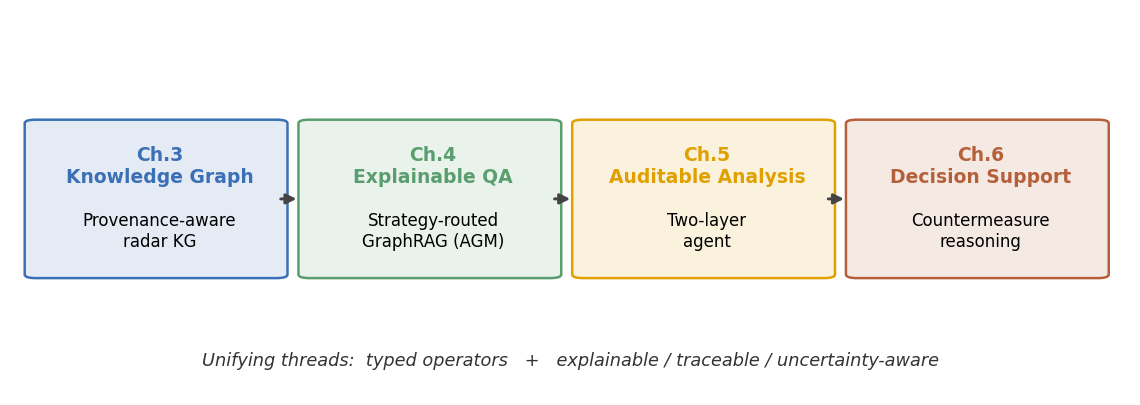
\includegraphics[width=0.78\textwidth]{fig1_roadmap}
\caption*{图 1-1　本文总体技术路线：构建知识图谱 → 可解释问答 → 可审计分析 → 对抗决策支持}
\end{figure}

\subsection*{1.5 论文组织结构}
\addcontentsline{toc}{subsection}{1.5 论文组织结构}

本文共七章，组织如下：

\begin{itemize}[leftmargin=2em]
\item \textbf{第一章 绪论。} 阐述研究背景与意义，综述国内外研究现状，凝练问题与挑战，概述本文工作与创新点。
\item \textbf{第二章 相关理论与技术基础。} 介绍知识图谱、检索增强生成与 GraphRAG、大模型推理与智能体范式，以及雷达情报与电子战的基础概念。
\item \textbf{第三章 雷达领域可溯源知识图谱构建。} 给出属性图模式、多源抽取流程与可溯源元数据设计，及知识图谱质量评估。
\item \textbf{第四章 策略路由的 GraphRAG 与答案-几何失配。} 提出 AGM 诊断、分发器与六类检索算子，并给出问答实验与消融分析。
\item \textbf{第五章 面向雷达情报的双层可审计分析智能体。} 给出算子组合执行器、ReAct 编排、可溯源报告与反思机制，及相应评测。
\item \textbf{第六章 面向雷达对抗的可解释决策支持。} 给出问题形式化、对抗本体与反制关系、确定性推理与可审计性、加权集合覆盖算法及战史校验。
\item \textbf{第七章 总结与展望。} 总结全文工作与创新，讨论局限与未来方向。
\end{itemize}



\section*{第二章 相关理论与技术基础}
\addcontentsline{toc}{section}{第二章 相关理论与技术基础}

本章介绍支撑全文的理论与技术：知识图谱及其属性图表示（§2.1）、检索增强生成与 GraphRAG（§2.2）、大语言模型推理与智能体范式（§2.3）、知识图谱问答方法（§2.4），以及雷达情报与电子战的基础概念（§2.5）。

\subsection*{2.1 知识图谱与属性图表示}
\addcontentsline{toc}{subsection}{2.1 知识图谱与属性图表示}

知识图谱是一种以图结构组织知识的方式，其基本单元是三元组 $(h, r, t)$，表示头实体 $h$ 与尾实体 $t$ 之间存在关系 $r$[1,2]。在数据模型上，常见有 RDF 三元组模型与\textbf{属性图}（Property Graph）模型两类：前者将一切表示为三元组，后者允许节点与边携带属性（键值对）。对雷达装备这类既有大量实体间关系（研制方、平台、衍生型号）又有大量数值/枚举属性（频段、探测距离、峰值功率）的领域，属性图模型更为自然：可将"型号—关系—型号/厂商/平台"建为边，将"频率、功率、年代"等建为节点属性，从而避免把属性强行表示为大量字面量尾节点所带来的边稀疏问题[1]。

形式化地，一个属性图可记为 $G=(V, E, A, \ell)$，其中 $V$ 为实体节点集，$E\subseteq V\times \mathcal{R}\times V$ 为带类型 $\mathcal{R}$ 的有向边集，$A$ 为属性赋值（$A(v,\cdot)$ 给出节点 $v$ 的属性），$\ell$ 为类型标注函数。知识图谱的\textbf{质量}通常从覆盖度、准确率与一致性等维度评估；在情报应用中，还需额外关注\textbf{可溯源性}——每条边/属性应能回溯到其来源与置信度，这一需求将在第三章通过为三元组附加来源/置信度/证据元数据来满足。

\subsection*{2.2 检索增强生成与 GraphRAG}
\addcontentsline{toc}{subsection}{2.2 检索增强生成与 GraphRAG}

大语言模型将知识隐式编码于参数中，存在知识陈旧与幻觉问题。检索增强生成（RAG）[4] 通过引入外部非参数化记忆：在生成前先检索与问题相关的文档片段作为上下文，使模型"有据而答"。其检索环节可采用稀疏检索（如 BM25）或稠密检索（如 DPR[18]）。RAG 显著缓解了开放域问答中的幻觉，但其检索单元是\textbf{扁平的文本片段}，难以表达与利用知识间的结构关联。

GraphRAG[5] 在 RAG 基础上引入知识图谱：通过图上的实体、关系与社区结构组织检索，特别适合需要跨多文档、多实体聚合的"全局性"问题（如面向语料的查询聚焦摘要）。相关方法的系统梳理见综述[11]。然而，现有 GraphRAG 大多采用\textbf{统一的检索流程}（如固定的子图扩展或社区摘要），隐含假设"所有问题以相同方式利用图结构"。本文第四章指出，这一假设在面对形态各异的问题时并不成立，并提出按问题形态路由到不同检索算子的解决方案。

\subsection*{2.3 大语言模型推理与智能体范式}
\addcontentsline{toc}{subsection}{2.3 大语言模型推理与智能体范式}

自预训练语言模型 BERT[31] 与大规模少样本学习模型 GPT-3[32] 以来，大语言模型在语言理解与生成上取得突破，并涌现出上下文学习与复杂推理能力。本文实现所用为 DeepSeek 系列大模型[30]。下面介绍与本文方法直接相关的两类推理范式。

\textbf{思维链（CoT）。} Wei 等人发现，在提示中引导模型显式生成中间推理步骤，可显著提升其在算术、常识与符号推理上的表现[9]。CoT 揭示了"过程可见"对复杂推理的价值，也为后续可解释推理奠定基础。

\textbf{ReAct 与工具调用。} Yao 等人提出的 ReAct[8] 将"推理"与"行动"交错：模型在生成推理（Thought）的同时产生动作（Action，如调用检索/计算工具），并根据观察（Observation）调整后续计划。这一范式使大模型从"一次性生成"升级为"可与环境交互的智能体"，成为多步任务求解的通用骨架。本文第五章的外层编排即采用手写的 ReAct 循环（以 JSON 动作交互，不依赖特定框架），以获得对执行流程的完全控制与可审计性。

\textbf{信任路径问题。} 智能体范式虽强大，但若关键事实由模型自由生成，则结论不可复现、不可审计。本文主张：在高可靠性应用中，应将大模型限定于"语言理解与表达"职能，而把"事实裁决"交由确定性组件完成——即大模型不进入关键事实的信任路径。该原则在第五、六章被分别实现并形式化。

\subsection*{2.4 知识图谱问答方法}
\addcontentsline{toc}{subsection}{2.4 知识图谱问答方法}

KGQA 方法大致分为三类[10]：

\begin{itemize}[leftmargin=2em]
\item \textbf{语义解析（Semantic Parsing）。} 将自然语言问题翻译为形式化查询（如 SPARQL、$\lambda$-DCS），在图谱上执行得到答案。优点是精确、可执行；缺点是对复杂/口语化问题的解析鲁棒性不足。
\item \textbf{信息检索（Information Retrieval）。} 检索与问题相关的子图或路径，再对候选答案排序。鲁棒性较好，但召回质量受检索策略影响大。
\item \textbf{大模型与知识图谱结合。} 以 RoG[6]、ToG[7] 为代表：RoG 先生成关系路径作为"忠实计划"再检索推理路径；ToG 将模型作为智能体在图上束搜索。这类方法兼顾了语言理解与结构推理，并强调忠实性与可解释性[3]。
\end{itemize}

本文方法与上述工作的关系是：在"检索/信息检索"路线内，进一步引入\textbf{问题形态分类与类型化算子}，使检索结构随问题几何而变（第四章）；并在问答之上叠加可组合执行与可审计编排（第五章），从而服务于更复杂的分析与决策需求。

\subsection*{2.5 雷达情报与电子战基础概念}
\addcontentsline{toc}{subsection}{2.5 雷达情报与电子战基础概念}

\subsubsection*{2.5.1 雷达体制与威胁画像}
\addcontentsline{toc}{subsubsection}{2.5.1 雷达体制与威胁画像}

雷达按用途可分为搜索/警戒、目标截获、跟踪、火控/制导等；按跟踪体制可分为圆锥扫描、波瓣切换、单脉冲、边扫描边跟踪（TWS）、连续波照射等[16]。其中\textbf{跟踪体制}对对抗方式具有决定性意义：圆锥扫描/序列波瓣依赖时序幅度比较测角，易受角度欺骗；而单脉冲在单个脉冲内完成测角，天然抗多数幅度类角度欺骗。雷达的工作频段、脉冲重复频率、有效辐射功率、是否频率捷变、是否低截获（LPI）等参数，共同构成其\textbf{威胁画像}，是对抗决策的输入（详见第六章）。

\subsubsection*{2.5.2 电子战：ESM、ECM 与 ECCM}
\addcontentsline{toc}{subsubsection}{2.5.2 电子战：ESM、ECM 与 ECCM}

电子战通常分为电子支援（ESM，截获识别敌方辐射）、电子攻击（ECM，干扰/欺骗）与电子防护（ECCM/EP，抗干扰）[13,15]。雷达对抗的典型流程是一条"侦察—识别—决策—行动—评估"的链路：先由 ESM 截获信号并比对威胁库确定型号（建立电子战斗序，EOB），再据其特征选择对抗手段并实施[15]。

\textbf{干扰（ECM）} 大致分为三类[13,15,22]：压制式（瞄准、拦阻、扫频噪声，抬高噪声底以降低探测距离）、欺骗式（距离门拖引 RGPO、速度门拖引 VGPO、倒相增益、交叉眼、交叉极化、DRFM 假目标等，制造虚假的距离/速度/角度信息）、以及无源（箔条、诱饵）。

\textbf{抗干扰（ECCM）} 则包括频率捷变、PRF 抖动、单脉冲测角、旁瓣对消/匿影、脉冲压缩、前沿跟踪、干扰源寻的、极化分集等[15,22]。干扰与抗干扰构成一对相互克制的"猫鼠博弈"：例如单脉冲克制倒相增益，前沿跟踪克制距离门拖引，极化分集克制交叉极化。第六章将这一克制关系形式化为\textbf{反制关系} $\mathcal{D}$，并据此进行确定性推理。

\subsubsection*{2.5.3 压制敌防空（SEAD）与认知电子战}
\addcontentsline{toc}{subsubsection}{2.5.3 压制敌防空（SEAD）与认知电子战}

压制敌防空（Suppression of Enemy Air Defenses, SEAD）是针对敌方防空体系（尤其是地空导弹的制导/预警雷达）的综合电子战行动，手段包括反辐射导弹硬摧毁、远距/随队干扰软压制、以及诱饵诱骗等[15]。这表明：\textbf{对抗的真实对象是敌方防空雷达}，而非己方平台雷达——这一认识直接决定了第六章威胁库的构建对象。

在智能化方面，认知电子战将干扰决策建模为（部分可观测）马尔可夫决策过程，采用强化学习自适应选择干扰策略[12]。这类方法长于在线对抗优化，但其决策为黑箱、依赖奖励信号且不可溯源。本文则走另一条互补路线：以\textbf{可解释、可审计、知识可溯源}的方式，基于威胁画像与电子战学理给出对抗建议，定位于情报辅助与决策支持，而非闭环干扰控制。

\subsection*{2.6 本章小结}
\addcontentsline{toc}{subsection}{2.6 本章小结}

本章梳理了知识图谱、检索增强生成与 GraphRAG、大模型推理与智能体、知识图谱问答，以及雷达情报与电子战的基础理论与方法。这些基础既揭示了通用方法在专业、可解释、面向决策场景下的不足，也为后续各章的设计提供了概念与工具支撑：属性图与可溯源元数据（第三章）、类型化检索算子（第四章）、可审计的算子组合与 ReAct 编排（第五章）、以及电子战学理的形式化与对抗推理（第六章）。



\section*{第三章 雷达领域可溯源知识图谱构建}
\addcontentsline{toc}{section}{第三章 雷达领域可溯源知识图谱构建}

知识图谱是后续问答（第四章）、分析（第五章）与对抗决策（第六章）的统一知识底座。本章针对雷达情报的领域特性，设计面向雷达装备的属性图模式（§3.2），给出多源知识抽取流程（§3.3）与可溯源元数据模型（§3.4），并对所构建图谱进行规模与质量评估（§3.5）。

\subsection*{3.1 概述与设计目标}
\addcontentsline{toc}{subsection}{3.1 概述与设计目标}

雷达情报具有三个对知识表示提出特殊要求的特性：（i）\textbf{实体—关系与实体—属性并重}：既有"型号—研制方—国家""型号—部署平台"等关系，又有"频段、探测距离、峰值功率、服役年代"等大量数值/枚举属性；（ii）\textbf{来源异构、可信度不一}：知识来自领域手册、公开百科、结构化知识库与规则推断，质量参差；（iii）\textbf{面向可信应用}：图谱将服务于情报问答与对抗决策，任一错误事实都可能沿推理链放大，故每条知识必须\textbf{可溯源}。

据此，本章的设计目标为：

\begin{itemize}[leftmargin=2em]
\item \textbf{G1 表达充分}：以属性图区分"实体间的边"与"实体上的属性"，避免将属性强行表示为大量字面量尾节点而造成的边稀疏（§3.2）。
\item \textbf{G2 多源可融合}：建立从非结构化手册、半结构化百科到结构化知识库的统一抽取与归一流程（§3.3）。
\item \textbf{G3 可溯源}：为每条声明附加来源、置信度与证据三元组，使任意查询结果可回溯（§3.4）。
\end{itemize}

\subsection*{3.2 雷达装备属性图模式}
\addcontentsline{toc}{subsection}{3.2 雷达装备属性图模式}

\subsubsection*{3.2.1 形式化定义}
\addcontentsline{toc}{subsubsection}{3.2.1 形式化定义}

沿用第二章的属性图定义，本文将雷达知识图谱建模为

\[G=(V,\,E,\,A,\,\ell,\,\mathrm{prov}),\]

其中 $V$ 为实体节点集，$E\subseteq V\times\mathcal{R}\times V$ 为带类型 $\mathcal{R}$ 的有向边集，$A:V\times \mathcal{K}\rightharpoonup \mathcal{U}$ 为节点属性赋值（$\mathcal{K}$ 为属性键集、$\mathcal{U}$ 为取值域），$\ell:V\to \mathcal{T}$ 为实体类型标注（$\mathcal{T}$ 为类型集），$\mathrm{prov}$ 为可溯源元数据函数（§3.4）。这一定义相对传统 RDF 三元组模型的关键区别在于：**属性 $A$ 与边 $E$ 分离**——把"频率、功率、年代"等内禀特征作为节点属性，而非退化为大量 \texttt{hasXxx} 字面量边。

\subsubsection*{3.2.2 实体类型与关系}
\addcontentsline{toc}{subsubsection}{3.2.2 实体类型与关系}

图谱的核心实体类型 $\mathcal{T}$ 包括：雷达系统（Radar）、子系统/部件（Subsystem/Component）、研制方（Manufacturer）、国家（Country）、平台（Platform，含舰载/机载/地面）、频段（FrequencyBand）、技术体制（TechType）、工作模式（RadarMode）、功能（Function）、武器（Weapon）、标准（Standard）等。关系 $\mathcal{R}$ 区分为"实体间的边"（如 \texttt{developedBy}、\texttt{operatedBy}、\texttt{countryOfOrigin}、\texttt{deployedOn}、\texttt{upgradeOf}、\texttt{compatibleWith}、\texttt{hasFrequencyBand}、\texttt{hasTechType}、\texttt{hasMode}、\texttt{hasFunction}、\texttt{hasSubsystem}、\texttt{meetsStandard} 等）与"应作为属性"的数值字段（如 \texttt{range\_km}、\texttt{frequency\_GHz}、\texttt{peak\_power\_kW}、\texttt{weight\_kg}、\texttt{year} 等）。表 3-1 列出代表性关系及其域—范围约束。

\textbf{表 3-1 代表性关系及其域—范围约束（节选）}

\begin{center}\small
\begin{tabular}{|p{0.307\textwidth}|p{0.307\textwidth}|p{0.307\textwidth}|}
\hline
\textbf{关系} & \textbf{域 → 范围} & \textbf{语义} \\ \hline
\texttt{developedBy} & Radar → Manufacturer & 研制方 \\ \hline
\texttt{countryOfOrigin} & Radar → Country & 原产国 \\ \hline
\texttt{operatedBy} & Radar → Country & 使用国 \\ \hline
\texttt{deployedOn} & Radar → Platform & 部署平台 \\ \hline
\texttt{hasFrequencyBand} & Radar → FrequencyBand & 工作频段（可多值） \\ \hline
\texttt{hasTechType} & Radar → TechType & 技术体制（如 AESA/脉冲多普勒） \\ \hline
\texttt{hasMode} / \texttt{hasFunction} & Radar → RadarMode/Function & 工作模式/功能（可多值） \\ \hline
\texttt{upgradeOf} / \texttt{derivedFrom} & Radar → Radar & 型号演化关系 \\ \hline
\texttt{compatibleWith} & Radar → Weapon & 武器兼容 \\ \hline
\end{tabular}
\end{center}

\begin{quote}\itshape 设计权衡：将"主要研制方/原产国"等单值字段同时以边与属性冗余存储——边用于反向查询与多跳推理（"某厂研制了哪些雷达"），属性用于高效的单跳读取（"某雷达原产国"）。\end{quote}

\subsection*{3.3 多源知识抽取流程}
\addcontentsline{toc}{subsection}{3.3 多源知识抽取流程}

图谱构建采用"抽取—归一—融合"的分阶段流程，如图 3-1 所示。

\begin{Verbatim}
                          图 3-1  多源知识抽取与融合流程
┌──────────────┐   ┌──────────────┐   ┌──────────────┐   ┌──────────────┐
│  领域手册PDF  │   │  公开百科文本 │   │  结构化知识库 │   │   规则/推断   │
│ (机载雷达手册)│   │  (Wikipedia)  │   │  (Wikidata)   │   │              │
└──────┬───────┘   └──────┬───────┘   └──────┬───────┘   └──────┬───────┘
       │ OCR+版面解析       │ 段落/信息框      │ SPARQL/对齐      │ 既有图谱派生
       ▼                   ▼                  ▼                  ▼
┌─────────────────────────────────────────────────────────────────────┐
│        大模型辅助抽取（模式受限 + 关系/属性约束 + 证据要求）           │
└───────────────────────────────┬─────────────────────────────────────┘
                                 ▼
        ┌───────────────  归一化层  ───────────────┐
        │  实体别名消解(双语)·频段/国家规范·数值单位 │
        └───────────────────┬──────────────────────┘
                            ▼
        ┌──────────  融合 + 可溯源元数据(来源/置信/证据)  ──────────┐
        │              merged_triples（属性图实例）                  │
        └────────────────────────────────────────────────────────────┘
\end{Verbatim}

各阶段要点如下：

\begin{itemize}[leftmargin=2em]
\item \textbf{手册抽取（pdf\_spec\_block / pdf\_narrative\_llm）。} 对领域手册做版面解析与 OCR，按"参数表块"与"叙述段落"分别抽取：前者以正则解析结构化字段，后者由大模型在模式约束下抽取关系与属性。
\item \textbf{百科与开放库（stage\_c\_llm / 联网补全）。} 对图谱未覆盖或字段缺失的型号，从公开百科获取文本并经大模型抽取，结果标注为联网来源、较低置信，与图谱主体显式区分。
\item \textbf{规则派生（enrich\_rule / 结构推断）。} 对可由既有图谱确定性派生的关系（如同平台部署的"协同部署"），以规则生成并标注规则来源，\textbf{与真实抽取严格区分}，避免以推断充当实证。
\item \textbf{归一化。} 经双语别名层消解实体（中英文及别名映射到规范实体），规范频段（单字母 S/X/L…）、国家（中文标准名）与数值单位。
\item \textbf{融合与去噪。} 合并多源三元组，剔除 OCR 残片与自循环等噪声，输出带元数据的属性图实例 \texttt{merged\_triples}。
\end{itemize}

\begin{quote}\itshape 抽取的\textbf{质量优先于数量}：本文在抽取链中明确拒绝"为提升边数而进行的规则灌注"，仅保留有据可溯的事实与显式标注的规则派生，这与情报应用对可信度的要求一致。\end{quote}

\subsubsection*{3.3.1 多智能体抽取与忠实度门控}
\addcontentsline{toc}{subsubsection}{3.3.1 多智能体抽取与忠实度门控}

图 3-1 中"大模型辅助抽取"环节若退化为单次提示调用，存在两点不足：一是抽取结果的忠实度缺乏显式校验，模型可能产出原文并不支持的声明；二是固定模式会丢弃模式外的重要事实。为此，本文将该环节细化为三个职责分离的智能体协作流水线：

\begin{itemize}[leftmargin=2em]
\item \textbf{抽取器（Extractor）}：在模式约束下从源文本抽取候选三元组，是产量主力。
\item \textbf{校验器（Critic）——忠实度门控}：逐条判定"尾值是否在原文中出现、是否被讹误"，拒绝无原文支撑者。其判定范围\textbf{严格限定于 value-in-text}，不对关系类型的"合理性"做二次判断——后者会误毙合法领域事实（见下文消融）。该门控同时以轻量词面形式用于受控模式扩展的补抽（§3.5）。
\item \textbf{模式提议器（Schema-Proposer）}：对现有关系无法承载的重要事实，提议候选新关系进入独立池，经人工审核后\textbf{受控}加入模式（而非自动注入类型核心），由此发现的关系缺口与落地结果见 §3.5。
\end{itemize}

\textbf{批判门控的消融（忠实度增益与其边界）。} 为厘清校验器的真实价值，本文在同一组文档上对照"是否经校验"与"输入是否含噪"（以 OCR 式降质模拟扫描手册），接地率一律对\textbf{干净原文}判定（真值）。结果如表 3-2。

\textbf{表 3-2　忠实度门控的消融（接地率对干净原文，按文档平均，n=30）}

\begin{center}\small
\begin{tabular}{|p{0.184\textwidth}|p{0.184\textwidth}|p{0.184\textwidth}|p{0.184\textwidth}|p{0.184\textwidth}|}
\hline
\textbf{输入} & \textbf{仅抽取器} & \textbf{+校验器} & \textbf{增益} & \textbf{产量变化} \\ \hline
干净 & 83\% & \textbf{88\%} & \textbf{+5.1pp} & 376→320 \\ \hline
含噪 & 81\% & 85\% & +3.4pp & 366→301 \\ \hline
\end{tabular}
\end{center}

由表 3-2 可得三点诚实结论：（i）\textbf{忠实度门控确实提升接地率}（干净 +5.1pp、含噪 +3.4pp），代价是约 15\% 的产量下降——即以召回换精度，这恰合可审计情报图谱"宁缺毋滥"的取向；（ii）\textbf{增益不随输入噪声上升}：词级噪声仅将抽取忠实度由 83\% 降至 81\%（模型可读穿错字），故门控的价值在于"忠实度—精度"而非"噪声恢复"；（iii）\textbf{校验范围决定成败}：当校验器越界去判断"关系类型是否合理"时，会误毙诸如"AMES Type 82 用于预警"这类正确事实，反而使接地率由 86\% 降至 82\%。据此本文采用\textbf{窄范围忠实度校验}，并将"模式合理性"交由提议器与人工审核处理，而非让校验器越权。

\begin{quote}\itshape 该多智能体分解的意义不在于堆叠模块，而在于\textbf{把"可信度"做成抽取流程内的一等机制}：校验器是 §3.4 可溯源模型中"证据—置信"得以成立的执行者，提议器则在不破坏类型约束的前提下持续扩展模式覆盖。\end{quote}

\subsection*{3.4 可溯源元数据模型}
\addcontentsline{toc}{subsection}{3.4 可溯源元数据模型}

为满足 G3，本文为每条声明 $x$（边或属性）附加可溯源三元组

\[\mathrm{prov}(x)=\big(\mathrm{source}(x),\ \mathrm{conf}(x)\in[0,1],\ \mathrm{evidence}(x)\big),\]

其中 $\mathrm{source}$ 标识抽取来源（如 \texttt{pdf\_spec\_block}、\texttt{stage\_c\_llm}、\texttt{enrich\_rule}、\texttt{wikipedia}），$\mathrm{conf}$ 为来源相关的置信度，$\mathrm{evidence}$ 为支撑该声明的原文片段或派生依据。该元数据贯穿后续各章：第五章据此生成逐条带来源与置信的情报报告，并对低置信事实显式标注；第六章据此实现来源分层的不确定性传播。

\begin{quote}\itshape \textbf{可溯源性的意义。} 在情报与决策场景中，"一个结论"远不如"一个可核验其来源与可信度的结论"有用。$\mathrm{prov}$ 使图谱从"知识的集合"升级为"可审计的知识"，这是本文区别于一般领域图谱的关键设计。\end{quote}

\subsection*{3.5 图谱规模与质量评估}
\addcontentsline{toc}{subsection}{3.5 图谱规模与质量评估}

最终构建的雷达知识图谱包含 \textbf{17 096} 条三元组（其中含 §3.3.1 模式提议器经受控扩展、忠实度门控补抽的 583 条新边，见下文）。图 3-2 给出三元组数量最多的 15 类关系：工作模式（\texttt{hasMode}）、功能（\texttt{hasFunction}）、研制方（\texttt{developedBy}）、子系统（\texttt{hasSubsystem}）、部署平台（\texttt{deployedOn}）等关系占据主体，反映了雷达装备"多模式、多功能、多部署"的领域特征；同时可见经属性化处理后，数值字段（如 \texttt{range\_km}）以适度规模并存，验证了 §3.2 属性图设计避免边稀疏的有效性。

\begin{figure}[htbp]\centering
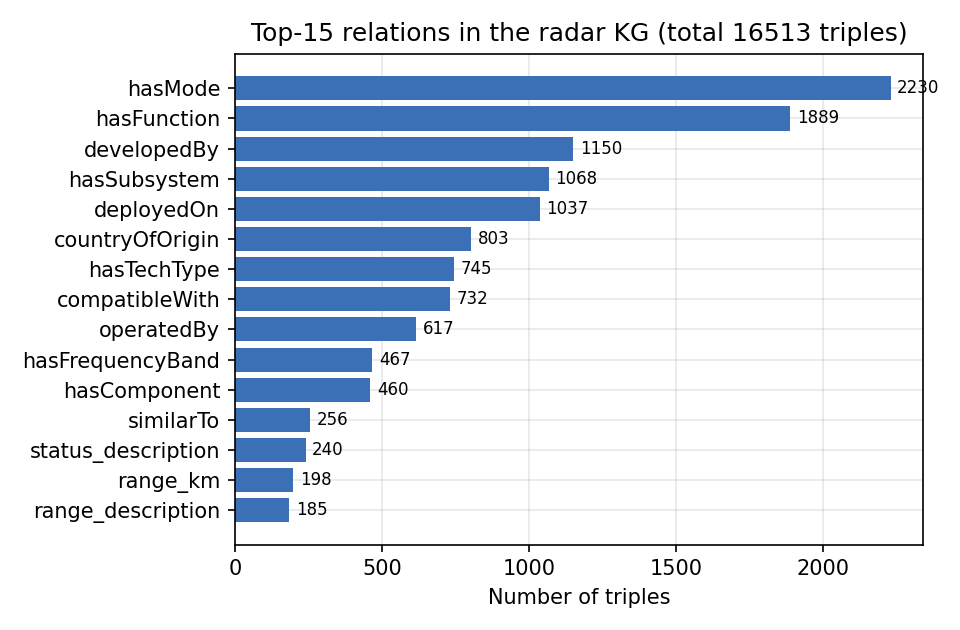
\includegraphics[width=0.78\textwidth]{fig3_relations}
\caption*{图 3-2　雷达知识图谱中数量最多的 15 类关系}
\end{figure}

图 3-3 给出按抽取来源统计的三元组分布：属性化字段（\texttt{v2\_attribute}）、结构化字段抽取（\texttt{extract\_std\_field}）、功能富化（\texttt{enrich\_func\_llm}）、手册叙述与参数块抽取（\texttt{pdf\_narrative\_llm}、\texttt{pdf\_spec\_block}）等构成主要来源。来源的多样性与可标注性，是 §3.4 可溯源模型得以落地的前提。

\begin{figure}[htbp]\centering
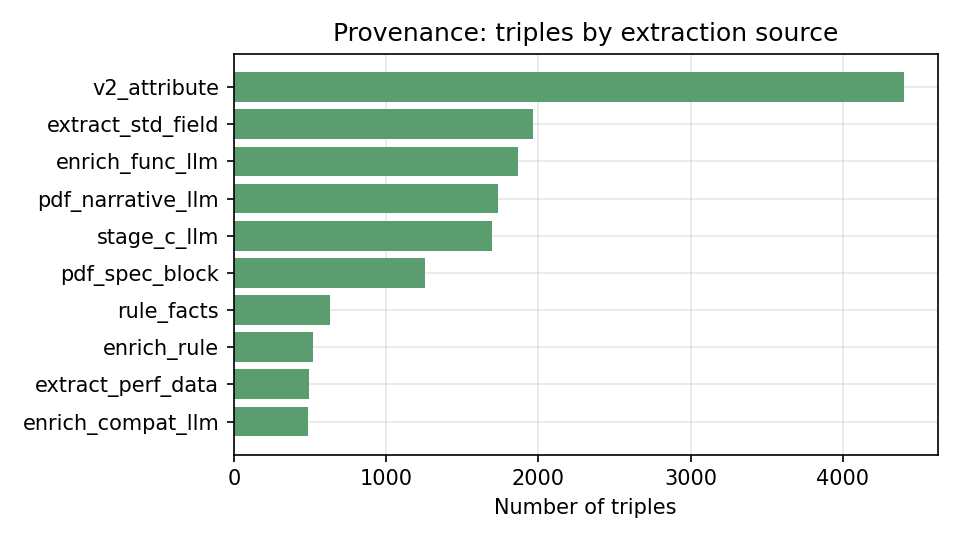
\includegraphics[width=0.78\textwidth]{fig3_sources}
\caption*{图 3-3　三元组按抽取来源的分布（Top-10）}
\end{figure}

在质量层面，本文沿可信知识图谱评估的标准维度（Zaveri 等的质量框架[33]）给出\textbf{可量化且诚实}的评估。需先厘清一个常被混淆的前提：\textbf{质量 ≠ 准确率}——准确率（事实对错）是唯一须以人工/独立金标判定的维度，而一致性、忠实度、印证度、覆盖度等均可由\textbf{无需金标的自动指标}度量。本文据此组织评估：\textbf{自动忠实度/一致性指标 + 独立交叉核验 + 任务式外在评估}，并辅以\textbf{领域专家分层抽样的人工金标准确率}（表 3-3，详见下文 (iv)）。尤其地，\textbf{忠实度（faithfulness，抽取是否忠于原文）与准确率（accuracy，事实是否为真）是两回事}：前者抓"模型有没有瞎编"，后者抓"原文/链接对不对"，本文区分报告。

\textbf{表 3-3　知识图谱质量评估（多维度）}

\begin{center}\small
\begin{tabular}{|p{0.230\textwidth}|p{0.230\textwidth}|p{0.230\textwidth}|p{0.230\textwidth}|}
\hline
\textbf{维度} & \textbf{方法} & \textbf{结果} & \textbf{需人工金标} \\ \hline
可溯源性 & 元数据覆盖率 & \textbf{100\%}（每条带来源/置信/证据） & 否 \\ \hline
一致性 & 类型签名违例 & \textbf{0.07\%}（12 条；原始 6.49\% 几为命名问题） & 否 \\ \hline
一致性 & 功能性冲突 / 噪声残片 & \textbf{222} 个头 / \textbf{3.2\%} & 否 \\ \hline
忠实度（字面） & 引文级字符串接地 & \textbf{81\%}（叙述 88\%／参数块 77\%）；门控补抽 \textbf{97\%} & 否 \\ \hline
忠实度（语义） & \textbf{NLI 蕴含判定}（样本 n=178） & 支持 \textbf{57\%}；较字符串 \textbf{+24 找回／−37 揪出} & 否 \\ \hline
\textbf{准确率（人工金标）} & 领域专家分层抽样（n=173，Gao'19[34]） & \textbf{85.1\%} 分层 95\%CI[75,95]／91\% 合并 & \textbf{是} \\ \hline
多源印证 & 独立来源投票 & 仅 \textbf{0.3\%} 被 ≥2 源印证（来源互补非冗余） & 否 \\ \hline
独立交叉核验 & Wikidata 比对 & 覆盖稀疏；\textbf{查出真实错误}（AN/APG-81/77 误标研制方） & 半（外部库） \\ \hline
任务式（外在） & RadarKG-QA-499（第四章） & \textbf{88.6\%} 可解释问答 & 外在指标 \\ \hline
覆盖度 & 受控模式扩展（§3.3.1） & \textbf{+583 边}，190 型号获新边 & 否 \\ \hline
\end{tabular}
\end{center}

\textbf{几点方法学说明与诚实结论：}

（i）\textbf{忠实度用语义而非字面度量。} 朴素字符串接地有两类错：把改写/翻译的正确事实误判为未接地（漏判），又把"字面出现但并不表达该关系"的错误事实误判为接地（误判）。本文以 NLI 蕴含判定（给裁判\textbf{原文}、只判是否支持，从而判读理解而非世界知识，缓解"以大模型评大模型图谱"的循环）取而代之：样本上它找回 24 条字符串漏判、揪出 37 条字符串误判，且\textbf{揪出多于找回}，说明\textbf{字符串接地高估了忠实度}；NLI 支持率 57\% 是更硬的下界（引文片段常较短，含欠完整引文与少量裁判误判）。该指标对\textbf{本文自身新增的模式扩展边同样有效}（揪出了一条可疑的 \texttt{replaces} 边），体现评估的中立性。

（ii）\textbf{多源投票在本图谱不适用，反证置信分层的合理性。} 四个独立来源（百科/手册/Wikidata/GlobalSecurity）仅 0.3\% 的事实被 ≥2 源同时印证——它们\textbf{互补（覆盖不同型号）而非冗余}，故 Knowledge-Vault[35] 式跨源投票在此失效；这正说明 §3.4 的\textbf{逐源置信分层}比依赖跨源印证更契合本场景。

（iii）\textbf{以任务表现外在佐证图谱质量。} 第四章在 RadarKG-QA-499 上取得 88.6\% 的可解释问答准确率——图谱需足够准确、可溯源，方能支撑此结果，这是对图谱可用质量的外在证据。

（iv）\textbf{准确率：领域专家分层抽样的人工金标。} 本文摒弃"以大模型判大模型图谱"的循环式自评（弃用现成的 LLM 自动标注），改由领域专家按 Gao 等（VLDB'19）[34]的分层抽样对 \textbf{173 条}三元组逐条人工核对（每条附可核证据，核实率 99\%）。结果：\textbf{按各来源在全库占比加权的图谱准确率为 85.1\%（95\% CI [75.1\%, 95.0\%]）}，合并 Wilson 估计 90.7\%（[85.4\%, 94.2\%]）。二者之差恰揭示真相——\textbf{最大的来源层（数值属性，占库约三成）也是最弱层（精度 64\%）}，加权估计如实反映了这一点。\textbf{per-source 精度进而验证了 §3.4 的置信分层}：文本/结构化来源精度高（\texttt{stage\_c}、参数块、Wikidata、受控扩展均 92–100\%，其中 §3.3.1 新增边人工核验 \textbf{100\%}），数值/性能属性最弱（\texttt{v2\_attribute} 64\%、\texttt{extract\_perf\_data} 75\%）——"数值属性置信应下调"由此从推测升级为\textbf{人工金标证实}的结论。**尤须强调:单一 85\% 会掩盖层间差异,故本文按来源层分解报告(表 3-4)。抽取层普遍达 90–93\%,而属性摊平层仅 69\%;更关键的是,规则/推断富化层（占库约 25\%）按设计为低置信、本次未纳入金标标注——因此 85\% 是对可核验抽取部分（约占库 75\%）的加权准确率,\texttt{下游若不按 §3.4 置信分层过滤推断层,实际可用准确率将低于此值},这是须诚实声明的使用边界。**

\textbf{表 3-4　按来源层的人工金标准确率（诚实分层，避免单一数字掩盖层间差异）}

\begin{center}\small
\begin{tabular}{|p{0.307\textwidth}|p{0.307\textwidth}|p{0.307\textwidth}|}
\hline
\textbf{来源层} & \textbf{占库} & \textbf{人工精度} \\ \hline
手册（PDF/OCR 抽取） & 42\% & \textbf{93\%} \\ \hline
Wikidata & 2\% & 92\% \\ \hline
公开百科 LLM & 2\% & 90\% \\ \hline
受控 schema 扩展 & 3\% & 100\% \\ \hline
属性摊平（数值/描述） & 25\% & \textbf{69\%} \\ \hline
规则/推断富化 & 25\% & \textbf{未测（低置信，应过滤）} \\ \hline
\end{tabular}
\end{center}

（v）\textbf{错误类型学与自动指标的相互印证。} 对 16 条判错的归纳暴露出几类系统性错误，且与前述自动指标高度一致：①\textbf{张冠李戴}（APQ-120 的平台被误挂到 APQ-36/AWG-11）——正是 (i) 中 NLI 揪出的同型错误；②\textbf{收购方 ≠ 原研制方}（Northrop Grumman 记成原研 Westinghouse/Bendix）——正是独立 Wikidata 交叉核验发现的同型错误；③\textbf{关系混淆}（"吸取…经验"记为 \texttt{衍生自}、"developed \textit{for} …"记为研制方、机体承包商记为雷达研制方）；④\textbf{数值属性拼接/错值}；⑤\textbf{劣质头实体}（"ATR,"、地名 "Chelmsford" 被当作雷达型号）。\textbf{人工与自动评估在错误类型上的一致，构成相互印证}，并把改进重点明确指向数值属性与实体消解——后者经实测（确定性规范化在本图谱上弊大于利，原始计数本就接近金标、激进合并反误并不同型号）列为未来工作，而非以未经验证的方法粉饰指标。

（vi）\textbf{面向最弱层的数据清洗（方法与诚实边界）。} 承 (iv) 的诊断（数值属性层最弱，64\%，且错误集中于 \texttt{*\_description} 的 OCR 乱码片段），本文对该层实施分层清洗：\textbf{确定性层}安全删除 \textbf{187} 条"乱码描述 + 已有干净归一数值"的冗余错误副本（零信息损失，规范数值仍在）、修正若干劣质头与浮点，并将 \textbf{329} 条无干净副本的乱码片段\textbf{降置信}（而非删除或臆造，交由 §3.4 的置信过滤处理），图谱由 17 096 精简为 \textbf{16 909} 条，该层样本精度由 64\% 升至 70\%。进而尝试\textbf{大模型接地重抽}以修复乱码值，但经验证\textbf{几近不可行}：330 条乱码中仅 30 条的实体有语料源，最终仅 1 条通过接地门控——因这些乱码是手册细参数（脉宽、PRF、接收机、方位等），其清洁源（原始手册）不在语料中。\textbf{由此得到一个诚实边界：OCR 乱码的手册参数在缺原始手册时无法自动修复，正确处置是"删冗余 + 降权不可验证"，而非以模型臆造充数}——这与本文可信优先、如实区分有效与无效改进的取向一致。

这种"\textbf{区分忠实度与准确率、只报站得住的自动指标、诚实标注金标缺口、如实区分有效与无效改进}"的取向，与本文一以贯之的可信优先原则一致。

\subsection*{3.6 本章小结}
\addcontentsline{toc}{subsection}{3.6 本章小结}

本章面向雷达情报的领域特性，设计了实体—关系与实体—属性分离的属性图模式，给出了融合领域手册、公开百科、结构化知识库与规则派生的多源抽取流程，并提出为每条声明附加来源/置信度/证据的可溯源元数据模型。所构建图谱含 1.7 万余条三元组、来源多样且全部可溯源，并经多维度质量评估（一致性、忠实度、准确率）与受控模式扩展，为第四章的策略路由问答、第五章的可审计分析与第六章的对抗决策提供了统一、可信的知识底座。



\section*{第四章 策略路由的 GraphRAG 与答案-几何失配}
\addcontentsline{toc}{section}{第四章 策略路由的 GraphRAG 与答案-几何失配}

本章针对通用 GraphRAG 在专业领域问答中"检索结构与问题需求错配"的问题（第一章挑战 C1），提出并形式化\textbf{答案-几何失配}（Answer-Geometry Mismatch, AGM）现象（§4.2），据此设计由问题分发器与六类\textbf{类型化检索算子}构成的策略路由问答方法（§4.3、§4.4），并在自建领域基准上给出实验与消融分析（§4.5、§4.6）。

\subsection*{4.1 概述：Top-K 检索的隐含假设}
\addcontentsline{toc}{subsection}{4.1 概述：Top-K 检索的隐含假设}

主流 RAG/GraphRAG 的检索核心是 \textbf{Top-K}：以查询为锚，按表面相关度对候选（文本片段或子图）排序并取前 $K$ 个。这一机制隐含了一个关于\textbf{答案几何}的假设：

\begin{quote}\itshape \textbf{假设（Top-K 答案几何）。} 问题的答案是一个\textbf{小的、可由与查询的表面相关度排序得到的集合}。\end{quote}

该假设在事实型问答（如"某雷达的研制方是谁"）上成立，这也是 WebQSP、NaturalQuestions 等公开基准的主体形态。但在工业级、专业领域知识图谱上，大量问题的信息需求与该假设结构性地不相容。本章的出发点即是：\textbf{症结不在排序器的优劣，而在"用错了几何"}——修复之道不是更好的 Top-K，而是为每类信息需求配备恰当的算子。

\subsection*{4.2 答案-几何失配（AGM）诊断}
\addcontentsline{toc}{subsection}{4.2 答案-几何失配（AGM）诊断}

\subsubsection*{4.2.1 现象与定义}
\addcontentsline{toc}{subsubsection}{4.2.1 现象与定义}

借用数据库领域 OLTP/OLAP 的二分：Top-K 检索本质是一种 \textbf{OLTP 式点查}（定位少数最相关记录），而许多情报问题本质是 \textbf{OLAP 式聚合/集合运算}（计数、求交、求补、多跳合成、双侧对比）。当问题的信息需求属于后者时，再精的排序也无法以"取前 $K$"的几何把答案表达出来。

\begin{quote}\itshape \textbf{定义 4.1（答案-几何失配，AGM）。} 设问题 $q$ 的最小信息需求为满足其答案所必需的知识子集 $I(q)$。若不存在常数 $K$ 使得"按表面相关度排序的前 $K$ 个候选"能覆盖 $I(q)$，则称 $q$ 相对 Top-K 发生\textbf{答案-几何失配}。\end{quote}

\subsubsection*{4.2.2 Top-K 无法满足的信息需求类}
\addcontentsline{toc}{subsubsection}{4.2.2 Top-K 无法满足的信息需求类}

我们不依赖对失败样例的经验归纳，而是\textbf{枚举 Top-K 无法满足的信息需求类}，并为每类推导一个原语算子（§4.3）。表 4-1 给出这一推导。

\textbf{表 4-1　信息需求类、Top-K 失败原因与对应算子}

\begin{center}\small
\begin{tabular}{|p{0.230\textwidth}|p{0.230\textwidth}|p{0.230\textwidth}|p{0.230\textwidth}|}
\hline
\textbf{信息需求类} & \textbf{答案所需} & \textbf{Top-K 为何失败} & \textbf{对应算子} \\ \hline
身份/事实型 & 一条最匹配三元组 & （Top-K 即可满足） & \textbf{lookup} \\ \hline
无界枚举/计数 & 某关系的\textbf{完整}头/尾集 & $K$ 是上界，答案集可大于 $K$ & \textbf{exhaustive} \\ \hline
多约束求交 & $N$ 个关系头集的交 & 排序无法表达 AND，混淆信号 & \textbf{constrained-join} \\ \hline
补集/非成员 & 完整已知集 + 显式缺口 & 图谱只存正事实，缺失是非局部的 & \textbf{complement} \\ \hline
关系合成（$k\ge2$） & 保持跳跃结构的\textbf{路径} & Top-K 是扁平的，丢失跳边界 & \textbf{path-plan} \\ \hline
二元（集合级）对比 & \textbf{两侧}子图均显式且对齐 & Top-K 可能饿死一侧、无法对齐 & \textbf{dual-subgraph} \\ \hline
\end{tabular}
\end{center}

\begin{quote}\itshape \textbf{AGM 是基准分布的性质，而非 Top-K 本身的性质。} 公开基准系统性地\textbf{少采样}这些类（其分布以事实型为主），故 Top-K 在公开基准上"看似够用"；而工业/专业图谱系统性地\textbf{多采样}这些类（计数、枚举、约束筛选是情报常态），故 Top-K 在此系统性失效。这一观察解释了"通用方法在专业领域水土不服"的结构性根因，并可迁移到雷达之外的领域。\end{quote}

\subsection*{4.3 类型化检索算子套件}
\addcontentsline{toc}{subsection}{4.3 类型化检索算子套件}

基于表 4-1 的推导，本文设计六类算子。除 \texttt{lookup} 对应 Top-K 本就能满足的事实型外，其余五类各自满足一类 Top-K 无法满足的信息需求。算子在 KG-only 的执行器中实现，\textbf{不经大模型}，从而保证答案集合的确定性与可复现性。

\textbf{表 4-2　六类算子的形式化与实现机制}

\begin{center}\small
\begin{tabular}{|p{0.307\textwidth}|p{0.307\textwidth}|p{0.307\textwidth}|}
\hline
\textbf{算子} & \textbf{形式化} & \textbf{实现机制} \\ \hline
\texttt{lookup} & 取最匹配三元组 & BM25[27] + 双编码器(Sentence-BERT[28]) + RRF 融合 + 2 跳图扩展；（head, relation）参数命中时绕行 KG 直查 \\ \hline
\texttt{exhaustive} & $\{h\mid (h,r,t)\in\mathrm{KG}\}$，无 $K$ 截断 & 完整头/尾集枚举；空结果时等价类回退 \\ \hline
\texttt{constrained-join} & $\bigcap_i \mathrm{heads}(r_i,t_i)$ & $N$ 约束头集求交；\textbf{等价类回退}（交集为空时并入语义等价关系，如 \texttt{countryOfOrigin}$\cup$\texttt{operatedBy}），缓解多源抽取的子图割裂 \\ \hline
\texttt{complement} & 枚举 $\{t\mid(h,r,t)\in\mathrm{KG}\}$ 后显式判缺 & 标记空/非成员，使模型显式输出"否"而非臆造 \\ \hline
\texttt{path-plan} & 链式 $\mathrm{tails}_{r_1}\!\circ\cdots\circ\mathrm{tails}_{r_k}$ & 关系链 BFS，支持反向遍历 $r^{-1}$，返回终点集与完整边轨迹 \\ \hline
\texttt{dual-subgraph} & 对 $(A,B)$ 并行 $\mathrm{tails}$ + 集合运算 & 并行展开两实体子图，预计算 $A\cap B,\ A\setminus B,\ B\setminus A$ 并对齐呈现 \\ \hline
\end{tabular}
\end{center}

\texttt{lookup} 还充当分发器纠错的\textbf{安全回退}：被误路由的问题退化为标准混合检索，而非落入错误算子的空结果。

\subsection*{4.4 分发器与双语别名层}
\addcontentsline{toc}{subsection}{4.4 分发器与双语别名层}

\textbf{问题分发器}为一个零样本大模型路由器（实现采用 DeepSeek 系列大模型[30]）：给定问题类型学定义与少量示例，将"问题 → 类型 → 算子"映射。其路由准确率为 \textbf{93.0\%}。值得强调的是（§4.6 将以消融证明）：分发器的贡献近似为 0，\textbf{全部增益来自算子设计本身}——这与"问题在于几何而非排序"的论点一致。

\textbf{双语别名层}为一条五级级联（直接匹配 → 614 形态别名索引 → 频段归一 → 后缀剥离 → 等价类并合），处理工业中文图谱"英文模式、中文为主取值"的混合语言问题，是算子在真实领域数据上稳定执行的工程保障。

整体流程为"三段大模型 + 一段 KG 执行"：分发器（选算子）、解析器（抽实体与关系链）、回答器（将证据渲染为自然语言），而知识图谱\textbf{仅在执行器中被查询，从不经由大模型}。

\subsection*{4.5 领域基准 RadarKG-QA-499}
\addcontentsline{toc}{subsection}{4.5 领域基准 RadarKG-QA-499}

为暴露 AGM，本文构建 \textbf{RadarKG-QA-499} 基准：基于 RadarKG-v2（评测时为 16 513 条核心三元组、98 关系与属性、4 827 实体；§3.3.1 受控模式扩展新增的 583 条边为评测后增补，查询核心关系不受其影响，故不计入本基准），覆盖单跳、关系反查、计数、枚举、多跳桥接/链、属性筛选、否定/不可答、集合对比、干扰项等 11 个类别共 499 题；其 Count 类问题的中位基数为公开基准的 \textbf{3.4 倍}，并设 26 题双语 OOD 压力子集。该基准在分布上\textbf{显式过采样} AGM 类问题，从而能区分"真正解决了结构性失配"与"在事实型分布上刷分"。

\subsection*{4.6 实验与分析}
\addcontentsline{toc}{subsection}{4.6 实验与分析}

\subsubsection*{4.6.1 总体结果}
\addcontentsline{toc}{subsubsection}{4.6.1 总体结果}

在全部 499 题上，对比三种方法：Top-K 基线、RoG[6]（统一路径规划）与本文策略路由方法。结果如图 4-1 与表 4-3 所示。

\begin{figure}[htbp]\centering
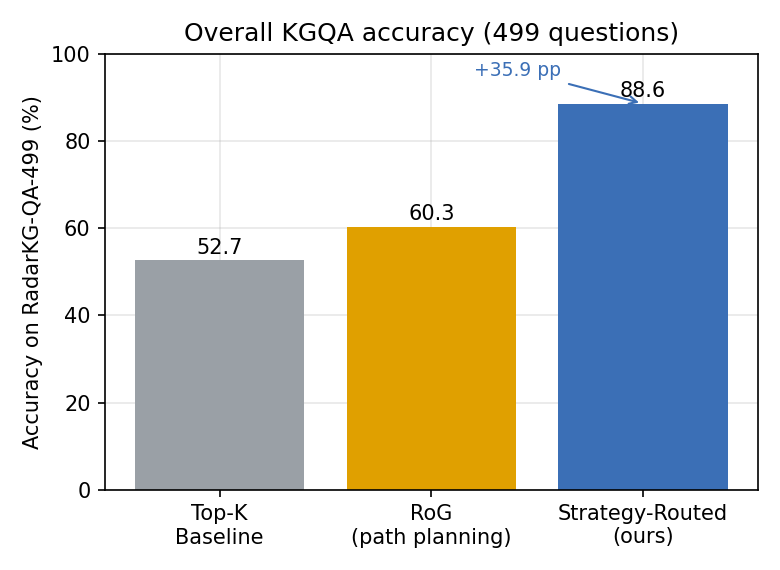
\includegraphics[width=0.78\textwidth]{fig4_qa_accuracy}
\caption*{图 4-1　RadarKG-QA-499 上的总体准确率（Baseline / RoG / 策略路由）}
\end{figure}

\textbf{表 4-3　总体与代表性类别准确率（\%，方括号为配对自举 95\% 置信区间）}

\begin{center}\small
\begin{tabular}{|p{0.153\textwidth}|p{0.153\textwidth}|p{0.153\textwidth}|p{0.153\textwidth}|p{0.153\textwidth}|p{0.153\textwidth}|}
\hline
\textbf{类别} & \textbf{题数} & \textbf{基线} & \textbf{RoG} & \textbf{策略路由} & \textbf{Δ(vs 基线)} \\ \hline
single\_hop & 80 & 83.8 & 11.2 & \textbf{86.2} & +2.5 \\ \hline
relation\_inverse & 50 & 40.0 & 74.0 & \textbf{86.0} & +46 \\ \hline
three\_hop\_chain & 30 & 23.3 & 50.0 & \textbf{93.3} & +70 \\ \hline
\textbf{总体} & \textbf{499} & \textbf{52.7} & \textbf{60.3} & \textbf{88.6} & \textbf{+35.9 [+32,+40]} \\ \hline
\end{tabular}
\end{center}

各代表性类别上基线与策略路由的对比如图 4-3 所示：在答案集结构性大于 $K$ 的类别（关系反查、三跳链）上，基线准确率极低而策略路由接近满分；在事实型的 \texttt{single\_hop} 上两者相当——这正是 AGM 论点的直观体现。

\begin{figure}[htbp]\centering
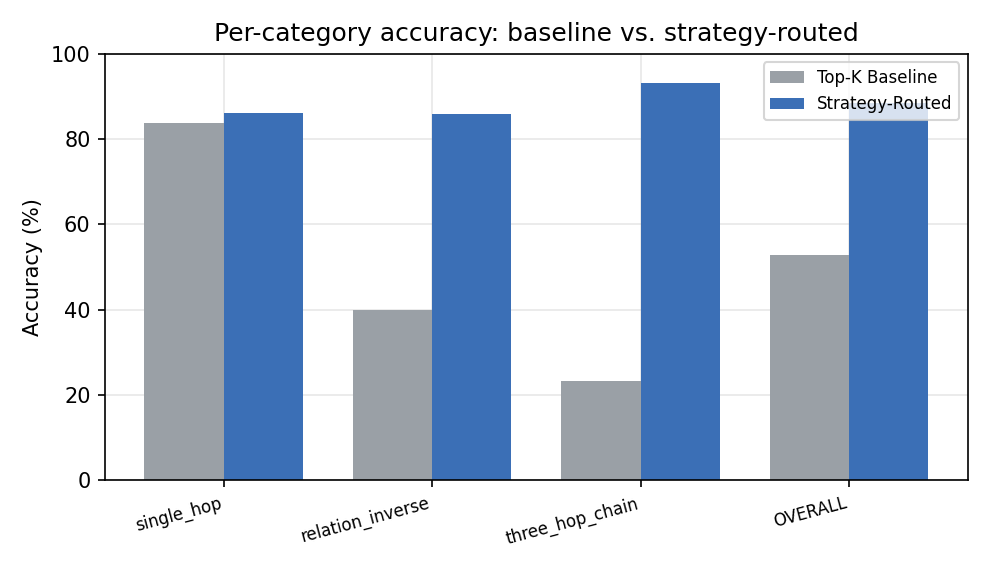
\includegraphics[width=0.78\textwidth]{fig4_per_category}
\caption*{图 4-3　代表性类别上的准确率对比（基线 vs 策略路由）}
\end{figure}

策略路由在 11 个类别中的 9 个以严格为正的置信区间取胜；其相对 RoG 亦提升 \textbf{+28.3 pp}。一个关键对照是：**RoG 在 \texttt{single\_hop} 上较基线下降 72.5 pp\textbf{——当问题本不需要路径时，统一的路径规划反而劣于不规划。这恰印证了本文论点：不存在普适的最优检索策略，}应按问题几何选择算子**。

\subsubsection*{4.6.2 增益来自算子还是分发器？}
\addcontentsline{toc}{subsubsection}{4.6.2 增益来自算子还是分发器？}

\textbf{Oracle 分发器消融。} 将大模型路由替换为"问题类型→算子"的金标准路由，端到端准确率为 \textbf{88.2\%}，与大模型路由（88.6\%）相差仅 0.4 pp。\textbf{分发器噪声的贡献近似为 0}，全部 +35.9 pp 增益由算子驱动。

\textbf{逐算子消融}（图 4-2）。强制各算子回退到 \texttt{lookup}，准确率下降分别为：去 \texttt{exhaustive} $-19$ pp、去 \texttt{path-plan} $-10$ pp、去 \texttt{constrained-join} $-8$ pp，而去 \texttt{complement}/\texttt{dual-subgraph} 在本基准分布上约 0 pp（\texttt{lookup}+大模型在该否定/对比分布上可优雅降级）。下降幅度与各算子所针对的 AGM 类一一对应（如去 \texttt{exhaustive} 使计数/枚举/关系反查各跌约 60 pp），验证了 §4.3 "算子↔失配类"的 1:1 推导。

\begin{figure}[htbp]\centering
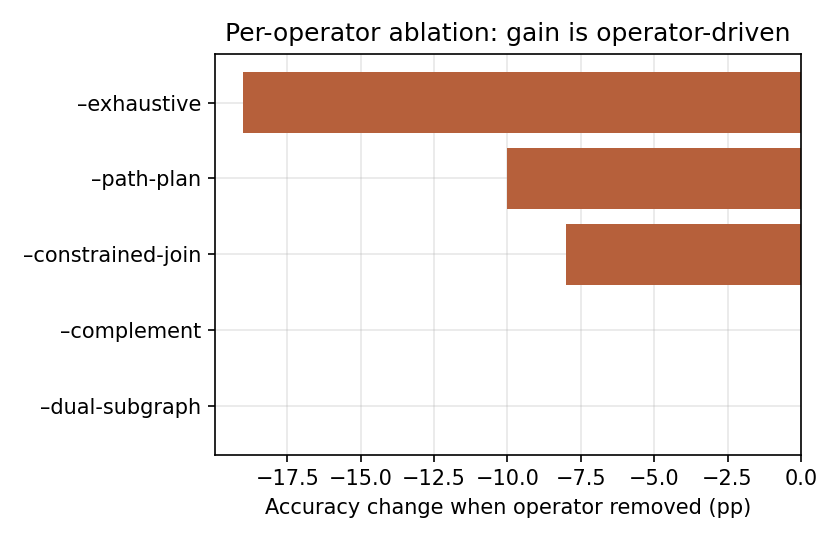
\includegraphics[width=0.78\textwidth]{fig4_ablation}
\caption*{图 4-2　逐算子消融：移除算子后的准确率变化}
\end{figure}

\textbf{检索预算消融。} 将基线的 $K{=}8$ 提升至 $K{=}20$ 仅使基线提升 +2.4 pp，策略路由相对 $K{=}20$ 基线仍领先 +33.5 pp。**增加检索预算无法修复"答案集结构性大于任何 $K$"的问题**——这证明 +35.9 pp 并非小 $K$ 造成的假象。

\textbf{套件规模消融。} 联合移除的下降近似线性叠加（如去 \texttt{exhaustive}+去 \texttt{path-plan} $\approx-29\,\mathrm{pp}=-19-10$），表明三个承重算子作用于\textbf{互不重叠}的问题切片；其中 \{lookup, exhaustive, path-plan, constrained-join\} 四算子子集在本基准上即可达到 94.0\% 的准确率，而仅 \texttt{lookup} 的下界为 57.0\%。

\subsection*{4.7 本章小结}
\addcontentsline{toc}{subsection}{4.7 本章小结}

本章提出并形式化了答案-几何失配（AGM）现象，借 OLTP/OLAP 框架揭示了通用 Top-K/GraphRAG 在专业领域系统性失效的结构性根因，并据"信息需求类"推导出六类类型化检索算子与一个轻量分发器。在显式暴露 AGM 的 RadarKG-QA-499 基准上，方法取得 88.6\% 的总体准确率，较基线 +35.9 pp、较 RoG +28.3 pp；一系列消融将增益精确定位到算子设计（分发器贡献约 0 pp），并验证了"算子↔失配类"的一一对应。本章的"类型化算子"思想，将在第五章被进一步发展为可组合、可审计的分析算子。



\section*{第五章 面向雷达情报的双层可审计分析智能体}
\addcontentsline{toc}{section}{第五章 面向雷达情报的双层可审计分析智能体}

第四章的策略路由解决了"单个问题用何种检索几何"的问题，但情报分析往往是\textbf{多步、组合、需产出可溯源情报产品}的任务（如"对比中美两型舰载雷达并生成档案"）。本章将单次问答升级为双层智能体（§5.2）：内层为类型化\textbf{算子组合执行器}（§5.3），外层为 ReAct 编排（§5.6）；并贯彻"大语言模型不进入信任路径"的可审计原则（§5.4），产出逐条可溯源的情报报告（§5.5）。最后给出评测（§5.7）。

\subsection*{5.1 概述：从问答到可审计分析}
\addcontentsline{toc}{subsection}{5.1 概述：从问答到可审计分析}

将第四章的问答能力推向分析，面临两个新要求：（i）\textbf{可组合}——复杂分析需把多个检索/集合运算组合成一个可确定性求值的整体，且中间实体不得在多次大模型转写中漂移；（ii）\textbf{可审计交付}——输出不应是一段可能含幻觉的叙述，而应是每条结论均挂"来源 + 置信度"的情报产品。为此本文提出双层架构，并把第四章的"类型化检索算子"发展为可嵌套组合的"分析算子"。

\subsection*{5.2 双层架构}
\addcontentsline{toc}{subsection}{5.2 双层架构}

系统分为内外两层，如图 5-1 所示。\textbf{外层}为手写的 ReAct[8] 编排循环：大模型每步输出一个 JSON 动作（调用某工具或结束），系统执行并回填观察，循环至给出最终回答。\textbf{内层}为类型化算子组合执行器：大模型仅产出一棵 JSON \textbf{计划树}，由确定性引擎递归求值，实体在树内传递、不经大模型二次转写。外层可调用的工具包括：组合查询（内层执行器）、可溯源装备档案、可溯源对比报告、图谱缺口联网补全。

\begin{Verbatim}
                     图 5-1  双层可审计分析智能体架构
  用户分析请求 / 多轮对话
        │  (多轮指代消解：将含指代的追问改写为自包含问题)
        ▼
 ┌──────────────────────────  外层：ReAct 编排循环  ──────────────────────────┐
 │  大模型每步输出 JSON 动作  →  执行工具  →  观察  →  循环  →  final            │
 │  工具：① 组合查询  ② 装备档案  ③ 对比报告  ④ 联网补全                          │
 │  交付：确定性 artifact（报告全文 + 逐条证据）原样呈现，大模型仅写引导语        │
 └───────────────────────────────────┬──────────────────────────────────────┘
                                      │ 工具①
                                      ▼
 ┌──────────────  内层：类型化算子组合执行器 + 计划器  ──────────────┐
 │  大模型出 JSON 计划树  →  确定性递归求值（实体在树内传递）           │
 │  算子：constraint / intersect / union / difference / path /        │
 │        count / enumerate / aggregate / compare / contains          │
 │  权威答案由确定性 trace 生成；空/退化结果触发反思重规划             │
 └────────────────────────────────────────────────────────────────────┘
\end{Verbatim}

\subsection*{5.3 内层：类型化算子组合执行器}
\addcontentsline{toc}{subsection}{5.3 内层：类型化算子组合执行器}

\subsubsection*{5.3.1 计划树文法}
\addcontentsline{toc}{subsubsection}{5.3.1 计划树文法}

第四章的六类检索算子是"扁平"的（每问一算子）。为支持组合分析，本章定义可嵌套的\textbf{计划树}文法 $\mathcal{G}$（节点即算子，子节点为其操作数）：

\[\begin{aligned}
\textit{Node} ::=\ & \mathtt{constraint}(r, v)\ \mid\ \mathtt{intersect}(N^{+})\ \mid\ \mathtt{union}(N^{+})\ \mid\ \mathtt{difference}(N, N)\\
\mid\ & \mathtt{path}(e, [r_1,\dots,r_k])\ \mid\ \mathtt{count}(N)\ \mid\ \mathtt{enumerate}(N)\\
\mid\ & \mathtt{aggregate}(f, a, N)\ \mid\ \mathtt{compare}(e_A, e_B, r)\ \mid\ \mathtt{contains}(N, e)
\end{aligned}\]

其中 $\mathtt{constraint}(r,v)$ 返回满足 $(?, r, v)$ 的实体集，$\mathtt{intersect}/\mathtt{union}/\mathtt{difference}$ 为集合运算，$\mathtt{path}$ 沿关系链（支持反向 $r^{-1}$）遍历，$\mathtt{count}/\mathtt{enumerate}$ 为基数/枚举，$\mathtt{aggregate}(f,a,\cdot)$ 对集合内实体的数值属性 $a$ 做聚合 $f\in\{\text{avg,sum,max,min}\}$，$\mathtt{compare}$ 对两实体某关系求同异，$\mathtt{contains}$ 判成员。该文法把第四章的检索原语提升为\textbf{可组合的代数}：例如"中国研制的 S 波段雷达有多少种"对应

\[\mathtt{count}\big(\mathtt{intersect}(\mathtt{constraint}(\texttt{countryOfOrigin},\text{中国}),\ \mathtt{constraint}(\texttt{hasFrequencyBand},\text{S}))\big).\]

\subsubsection*{5.3.2 确定性递归求值}
\addcontentsline{toc}{subsubsection}{5.3.2 确定性递归求值}

执行器对计划树做后序递归求值 $\mathrm{eval}:\textit{Node}\to (\textit{Value},\textit{Trace})$：叶子算子查询知识图谱，内部算子对子节点求值结果施加集合/数值运算，同时累积一棵\textbf{执行轨迹} $\textit{Trace}$（记录每步算子、输入、输出与命中的图谱事实）。关键性质是：\textbf{实体集合在树内以值传递}，不经大模型在中间步骤重新生成，从而杜绝了多步转写导致的"实体漂移"。

\begin{quote}\itshape \textbf{命题 5.1（组合求值的确定性）。} 给定知识图谱 $G$ 与计划树 $P\in\mathcal{G}$，$\mathrm{eval}(P)$ 的取值与轨迹是 $G$ 与 $P$ 的确定性函数，与任何大模型采样无关。\end{quote}
\begin{quote}\itshape \end{quote}
\begin{quote}\itshape \textit{证明概要.} 叶子算子是对 $G$ 的确定性查询；内部算子为集合/数值的确定性运算；递归复合保持确定性。$\square$\end{quote}

\subsection*{5.4 可审计性：大模型不进入信任路径}
\addcontentsline{toc}{subsection}{5.4 可审计性：大模型不进入信任路径}

设单次组合查询的输出为 $(\delta(P),\ \psi)$，其中\textbf{权威答案} $\delta(P)$ 由执行轨迹按确定性规则生成（如计数题输出"共 $n$ 款"、聚合题输出"$f(a)=x$（覆盖率 $c$）"），$\psi$ 为大模型对 $\delta(P)$ 的自然语言复述。

\begin{quote}\itshape \textbf{定理 5.2（分析答案的可审计性）。} 权威答案 $\delta(P)$ 是 $(G,P)$ 的确定性函数（命题 5.1）；大模型仅作用于 $\psi$，且 $\psi$ 被约束为对 $\delta(P)$ 的复述，不得增删数字与实体。故系统输出的\textbf{事实正确性不依赖大模型的事实性}，且可逐步回溯至图谱事实。\end{quote}

该定理的工程含义在一处典型故障中得到验证：早期实现让大模型直接读执行结果作答时，曾把"覆盖率 100 条"误述为"100\%"；将 $\delta(P)$ 设为权威答案、大模型仅复述后，此类错误被根除。\textbf{把不确定的生成式组件移出关键事实的信任路径}，是本文在第五、六章一以贯之的架构原则。

\subsection*{5.5 可溯源情报报告}
\addcontentsline{toc}{subsection}{5.5 可溯源情报报告}

外层工具产出两类可溯源情报产品：\textbf{装备档案}（单型号）与\textbf{对比报告}（双型号）。其设计要点：

\begin{itemize}[leftmargin=2em]
\item \textbf{逐条引证}：报告中每条事实均由图谱确定性渲染，并附其来源与置信度，形如"研制方：×××〔来源:pdf\_spec\_block，置信:0.90〕"。
\item \textbf{低置信过滤}：对置信度低于阈值（默认 0.75）的事实显式标注"⚠低置信"，且\textbf{不纳入}大模型自动概述，仅高置信事实参与概述生成；报告末尾汇总低置信条数，提示人工核验。
\item \textbf{概述可溯源校验}：对大模型生成的概述做轻量校验——其中出现的实体/数值 token 必须能在被引证事实中找到来源，否则计为"未溯源"。该校验把"概述忠实性"变为可度量指标（§5.7）。
\end{itemize}

\begin{quote}\itshape 这与定理 5.2 一致：报告的事实层完全由图谱确定性生成，大模型仅在受约束、且仅可见高置信事实的条件下做语言组织。\end{quote}

\subsection*{5.6 外层编排、反思与多轮}
\addcontentsline{toc}{subsection}{5.6 外层编排、反思与多轮}

\textbf{ReAct 编排}：外层以手写循环实现（JSON 动作，不依赖特定框架），便于对执行流程做完全控制与审计；最终回答阶段，系统将确定性 artifact（报告全文与逐条证据）\textbf{原样附加}，大模型仅写一句引导语，避免其在交付环节引入幻觉。

\textbf{反思重规划}：当内层执行返回空/退化结果时，系统并不直接作答，而是触发反思节点——以图谱中该关系的\textbf{真实取值}作为线索，提示计划器修正（如把约束值"在役"改为图谱实际存储的"服役中"），并重新求值。该机制以"图谱真实取值"为锚校正计划，1 轮即可修复多数取值不匹配类错误。

\textbf{多轮指代消解}：对含指代或省略的追问（"它的研制方呢？"），系统先依据对话历史将其改写为自包含问题（"AN/TPY-2 的研制方是谁？"）再进入执行，从而支持多轮分析对话。

\subsection*{5.7 评测}
\addcontentsline{toc}{subsection}{5.7 评测}

\textbf{组合能力。} 构造 72 题组合评测集（6 类各 12 题，金标准由执行器在图谱上算出），评测计划有效率、执行成功率与正确率。结果：计划有效率 100\%、执行成功率 100\%、\textbf{正确率 99\%}（聚合/对比/差集/多重计数/多重枚举类 100\%，两跳计数 92\%）。这些均为单算子流水线无法表达的组合题。

\textbf{报告可审计性。} 在 30 份装备档案上评测：确定性事实的引证覆盖率为 \textbf{100\%}（458/458 条均带来源）；大模型概述的可溯源率（token 级校验）均值为 \textbf{100\%}（24/24 份零编造）。主要评测指标汇总于图 5-2。

\begin{figure}[htbp]\centering
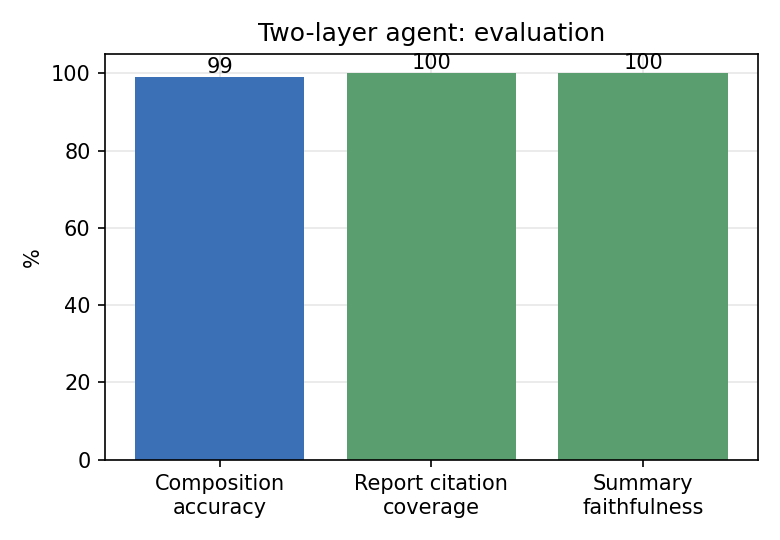
\includegraphics[width=0.78\textwidth]{fig5_agent_eval}
\caption*{图 5-2　双层智能体的组合正确率、报告引证覆盖率与概述可溯源率}
\end{figure}

\textbf{功能验证。} 反思节点在 1 轮内修复取值不匹配类的空结果，且不误触发正常查询；多轮指代消解正确改写追问；联网补全可在图谱未收录某型号时填补缺口并标注"未经图谱核验"。

\subsection*{5.8 本章小结}
\addcontentsline{toc}{subsection}{5.8 本章小结}

本章将单次问答升级为双层可审计分析智能体：内层以可嵌套的类型化算子组合执行器实现确定性组合求值（命题 5.1），外层以手写 ReAct 编排多步分析；并将"大模型不进入信任路径"形式化为可审计性定理（定理 5.2），据此产出逐条可溯源、低置信显式标注的情报报告。评测表明组合正确率 99\%、报告引证覆盖与概述可溯源率均为 100\%。本章的"可组合 + 可审计"思想，将在第六章被进一步用于构造面向对抗决策的推理算子。



\section*{第六章 面向雷达对抗的可解释决策支持}
\addcontentsline{toc}{section}{第六章 面向雷达对抗的可解释决策支持}

\begin{quote}\itshape 本章将系统从"雷达情报问答"推进到"雷达对抗决策辅助"：给定敌方防空雷达布控，输出\textbf{应采用何种干扰手段、应避免何种手段、如何应对其抗干扰、并以何种最小装备集合覆盖整个威胁群}的建议。与第三、四章的检索式问答不同，本章面对的是一个\textbf{带不确定性、知识稀疏且高度异构}的决策问题。我们的核心立场是：在这种领域，系统的价值不在于"给出一个答案"，而在于\textbf{给出一个可解释、可溯源、其不确定性被显式建模的答案}。为此本章给出对抗决策问题的形式化、对抗知识的可信度分层表示、确定性可审计推理算子，以及将战场级方案归约为加权集合覆盖的近似算法。\end{quote}


\subsection*{6.1 引言与问题动机}
\addcontentsline{toc}{subsection}{6.1 引言与问题动机}

\subsubsection*{6.1.1 从问答到决策的跃迁}
\addcontentsline{toc}{subsubsection}{6.1.1 从问答到决策的跃迁}

第三、四章的图谱问答回答的是"是什么"(What)——某雷达的参数、某国研制了哪些雷达。而作战层面真正的需求是"怎么办"(What to do)：\textbf{面对敌方防空体系，我方该如何对抗}。这类问题具有三个本质区别：

\begin{itemize}[leftmargin=2em]
\item \textbf{答案不是图谱中的一个节点，而是一个需要推导的方案}。它不存在于任何单一三元组中，必须由"威胁特征 + 对抗学理(doctrine)"合成。
\item \textbf{知识高度稀疏且涉密}。逐型号的实战对抗弱点多为机密；开源可得的是 doctrine 级(教科书级)的一般规律与少量已解密战史。
\item \textbf{不确定性是一等公民}。威胁画像本身可能是推断的、效能判断是启发式的——一个负责任的系统必须\textbf{显式携带并传播这些不确定性}，而非掩盖。
\end{itemize}

\subsubsection*{6.1.2 本章贡献}
\addcontentsline{toc}{subsubsection}{6.1.2 本章贡献}

\begin{itemize}[leftmargin=2em]
\item \textbf{（1）形式化}：将雷达对抗决策形式化为知识图谱上的推导问题，给出对抗本体 (jamming/ECCM) 与 \texttt{defeats} 反制关系的代数刻画(§6.2、§6.5)。
\item \textbf{（2）可信度分层}：提出三层来源的证据模型与置信度演算，使每条结论可回溯到"文献证据 / 学理推断 / 实战记载"三类来源之一(§6.3)。
\item \textbf{（3）软健全性抽取}：以"引文校验"作为抽取的软健全性过滤器，并以一个良序的填空式合并保证多来源融合无冲突(§6.4)。
\item \textbf{（4）可审计推理}：给出三分输出(可行/否决/被抵消)的确定性推理算子，并证明其\textbf{可审计性}——结论的事实部分仅由确定性 trace 决定，大语言模型不进入信任路径(§6.5)。
\item \textbf{（5）算法}：将战场级对抗方案归约为加权集合覆盖，给出贪心算法及其 $H_n$ 近似保证，并据此定义"干扰样式经济性"与"能力缺口"分析(§6.6)。
\item \textbf{（6）实证校验}：以已解密战史作为独立 ground truth 校验推理与学理的一致性，并量化"结论多样性"以验证系统克服了规则坍缩(§6.7、§6.8)。
\end{itemize}


\subsection*{6.2 问题形式化}
\addcontentsline{toc}{subsection}{6.2 问题形式化}

\subsubsection*{6.2.1 威胁雷达与威胁画像}
\addcontentsline{toc}{subsubsection}{6.2.1 威胁雷达与威胁画像}

设威胁雷达集合为 $\mathcal{R}$。每部雷达 $r\in\mathcal{R}$ 由一个\textbf{威胁画像} (threat profile) 刻画，它是定义在属性集 $\mathcal{A}$ 上的部分函数

\[\pi(r):\ \mathcal{A}\ \rightharpoonup\ \bigcup_{a\in\mathcal{A}}\mathrm{dom}(a),\]

其中关键属性及其论域为：用途 $\mathsf{purpose}\in\{\text{search, acquisition, track, fire\_control, SAM\_guidance, GCI, AEW, early\_warning,}\dots\}$、跟踪体制 $\mathsf{track}\in\{\text{monopulse, conical\_scan, lobe\_switching, TWS, range\_gate, cw\_illuminator, none}\}$、扫描方式、频段 $\mathsf{band}$、频率 $\mathsf{freq}\in\mathbb{R}_{>0}$、峰值功率、捷变标志 $\mathsf{agile}\in\{0,1\}$、低截获标志 $\mathsf{lpi}$、以及已采用的抗干扰技术集合 $\mathsf{eccm}\subseteq E$。"部分函数"刻画了一个关键现实：\textbf{画像往往不完整}，某些属性对某些雷达是未知的。

\subsubsection*{6.2.2 对抗本体}
\addcontentsline{toc}{subsubsection}{6.2.2 对抗本体}

定义两个本体集合：

\begin{itemize}[leftmargin=2em]
\item \textbf{干扰技术} $J$（jamming techniques），含压制类(瞄准/拦阻/扫频噪声)、欺骗类(距离门拖引 RGPO/RGPI、速度门拖引 VGPO、倒相增益、交叉眼、交叉极化、编队/闪烁、DRFM 假目标)与无源类(箔条、诱饵)；
\item \textbf{抗干扰技术} $E$（ECCM），含频率捷变、PRF 抖动、单脉冲、旁瓣对消/匿影、脉冲压缩、前沿跟踪、干扰源寻的、极化分集等。
\end{itemize}

二者通过\textbf{反制关系} (counter relation) 联系：

\[\mathcal{D}\ \subseteq\ E\times J,\qquad (e,j)\in\mathcal{D}\iff \text{抗干扰技术 }e\text{ 能挫败干扰技术 }j .\]

例如 $(\text{单脉冲},\ \text{倒相增益})\in\mathcal{D}$、$(\text{前沿跟踪},\ \text{RGPO})\in\mathcal{D}$、$(\text{极化分集},\ \text{交叉极化})\in\mathcal{D}$。记 $\mathcal{D}(e)=\{j:(e,j)\in\mathcal{D}\}$ 为 $e$ 所克制的干扰集合。$\mathcal{D}$ 是一个非对称、非传递的二部关系——它正是对抗"猫鼠博弈"的代数骨架。

\subsubsection*{6.2.3 学理规则与决策问题}
\addcontentsline{toc}{subsubsection}{6.2.3 学理规则与决策问题}

\textbf{学理知识}表示为带出处的规则集 $\mathcal{P}$。每条规则

\[\rho=\big(\mathrm{cond}_\rho,\ \mathrm{rec}_\rho,\ \mathrm{avoid}_\rho,\ c_\rho,\ \mathrm{src}_\rho\big),\]

其中 $\mathrm{cond}_\rho$ 是定义在画像上的合取谓词，$\mathrm{rec}_\rho\subseteq J$ 为推荐干扰集，$\mathrm{avoid}_\rho\subseteq J$ 为应避免集，$c_\rho\in[0,1]$ 为该条学理的置信度，$\mathrm{src}_\rho$ 为文献出处。

\begin{quote}\itshape \textbf{单威胁对抗决策问题。} 给定威胁 $r$ 与对抗本体 $(J,E,\mathcal{D},\mathcal{P})$，求一个三元划分 $\big(\mathrm{Viab}(r),\ \mathrm{Cnt}(r),\ \mathrm{Avoid}(r)\big)$ 及置信度赋值 $c(\cdot\,|\,r)$，使得每个判定都可回溯到 $\mathcal{P}$ 中的具体规则与 $r$ 的画像证据。\end{quote}

\begin{quote}\itshape \textbf{战场级对抗决策问题。} 给定威胁集合 $T\subseteq\mathcal{R}$ 及我方装备集 $\mathcal{S}$，在"装备-威胁可交战"约束下，求覆盖高威胁的\textbf{最小装备子集}与按手段的资源分配(见 §6.6)。\end{quote}

本章的工作即是为以上两个问题给出\textbf{可解释、可审计}的求解机制。


\subsection*{6.3 对抗知识的表示与可信度分层}
\addcontentsline{toc}{subsection}{6.3 对抗知识的表示与可信度分层}

领域的稀疏与异构使得"所有知识同等可信"成为危险假设。我们引入\textbf{来源分层} (provenance tiers)：每一条事实或属性取值 $x$ 都附带一个三元组

\[\mathrm{prov}(x)=\big(\mathrm{tier}(x),\ \mathrm{src}(x),\ c(x)\big),\qquad \mathrm{tier}(x)\in\{\textsf{evidence},\ \textsf{doctrine},\ \textsf{prior}\}.\]

\begin{itemize}[leftmargin=2em]
\item $\textsf{evidence}$：有文献/手册原文支撑(关键词命中或带引文的抽取)，置信度高($\approx 0.75\!-\!0.9$)；
\item $\textsf{prior}$：由学理先验推断(如"火控雷达通常单脉冲")，置信度低($\approx 0.45\!-\!0.55$)，在输出中显式标注为"推测"；
\item $\textsf{doctrine}$：来自已解密战史的实战记载(§6.7)，是唯一的型号级真实 ground truth。
\end{itemize}

知识库分三部分实现：(i) 机器可读的 doctrine 映射(干扰/抗干扰本体 + $\mathcal{D}$ + 规则 $\mathcal{P}$，每条带出处)；(ii) 威胁雷达库(89 部、9 国、30 余个防空体系，源自世界装备指南 WEG、Air Power Australia、GlobalSecurity、Wikipedia 等公开源，逐字段标注来源)；(iii) 我方电子战装备库(干扰机/诱饵/反辐射，带频段与支持的干扰样式)。

\begin{quote}\itshape \textbf{设计原则（可信度单调性）。} 任何下游推导的结论置信度不超过其依赖的最弱前提：$c(\text{结论})\le \min_i c(\text{前提}_i)$。这保证了"推测"前提不会被推导过程"洗白"成高置信结论——这是对领域不确定性的诚实传播。\end{quote}


\subsection*{6.4 威胁画像的分层抽取}
\addcontentsline{toc}{subsection}{6.4 威胁画像的分层抽取}

威胁画像中的判别性字段(跟踪体制、捷变、所采用 ECCM)在开源中稀疏。我们设计三层抽取，并以\textbf{填空式合并}(fill-missing)融合，按来源可信度排序，\textbf{只填未知字段}。

\subsubsection*{6.4.1 三层抽取}
\addcontentsline{toc}{subsubsection}{6.4.1 三层抽取}

\begin{itemize}[leftmargin=2em]
\item \textbf{T1 关键词层}：在已结构化的图谱文本上做确定性匹配(如"单脉冲""频率捷变")，命中即赋值，$\mathrm{tier}=\textsf{evidence}$。
\item \textbf{T2 大模型抽取层}：对仍缺字段且有充分文本(语料/联网)的雷达，调用大模型抽取，但\textbf{强制要求给出原文逐字引文}，并施加引文校验(下文)，$\mathrm{tier}=\textsf{evidence}$。
\item \textbf{T3 学理先验层}：仍缺失的字段由 §6.2 的学理先验填补(如 $\mathsf{purpose}\in\{\text{fire\_control}\}\Rightarrow\mathsf{track}=\text{monopulse}$)，$\mathrm{tier}=\textsf{prior}$，置信度压低。
\end{itemize}

\subsubsection*{6.4.2 引文校验作为软健全性过滤}
\addcontentsline{toc}{subsubsection}{6.4.2 引文校验作为软健全性过滤}

设大模型对字段 $a$ 给出取值 $v$ 与引文 $q$，源文本为 $\mathcal{T}$。定义\textbf{接受谓词}

\[\mathrm{Accept}(v,q,\mathcal{T})\ \equiv\ \big(v\ne\bot\big)\ \wedge\ \big(\mathrm{normalize}(q)\ \sqsubseteq\ \mathrm{normalize}(\mathcal{T})\big),\]

其中 $\sqsubseteq$ 为(归一化后的)子串关系。不满足者一律丢弃。该过滤器给出一个\textbf{相对健全性}保证：

\begin{quote}\itshape \textbf{命题 6.1（抽取的相对健全性）。} 在大模型如实复制引文(即引文确为其判断依据)的前提下，任何被接受的取值 $v$ 都存在源文本中的字面证据 $q\sqsubseteq\mathcal{T}$ 支撑之。因此引文校验排除了"无源臆造"(hallucination without textual support)进入画像。\end{quote}

\textit{证明概要.} 由 $\mathrm{Accept}$ 定义，被接受即蕴含 $q\sqsubseteq\mathcal{T}$ 且 $q$ 非空；故 $v$ 在 $\mathcal{T}$ 中有对应文本。"相对"指其健全性条件化于大模型不伪造引文——该条件可被进一步以更强校验(如语义蕴含判定)收紧。$\square$

该机制在实现中拦截了无引文支撑的抽取(实测对跟踪体制/扫描方式字段丢弃率非平凡)，并能跨语言校验(中、英引文均可)。

\subsubsection*{6.4.3 填空式合并的良序性}
\addcontentsline{toc}{subsubsection}{6.4.3 填空式合并的良序性}

三层在属性上诱导一个偏好序 $\textsf{evidence}\ \succ\ \textsf{prior}$，T1、T2 同属 $\textsf{evidence}$ 但按"先到先得"。合并算子 $\mathrm{merge}$ 对每个属性按 $\langle\text{T1, T2, T3}\rangle$ 顺序、\textbf{仅在该属性尚空时}赋值。

\begin{quote}\itshape \textbf{命题 6.2（合并无冲突且确定）。} $\mathrm{merge}$ 是良定义的函数：每个属性至多被赋值一次，结果与三层内部的并行处理顺序无关；且最终每个属性的来源层 $\mathrm{tier}$ 唯一确定。\end{quote}

\textit{证明概要.} "仅在尚空时赋值"使每属性的赋值发生在偏好序的首个非空层，后续层对该属性为幂等空操作；故赋值唯一、与层内顺序无关。$\square$

命题 6.2 的意义在于：多来源融合\textbf{不会产生需要仲裁的冲突}，从而避免了不可解释的"投票黑箱"——每个字段的取值、来源、置信都是确定且可展示的。


\subsection*{6.5 确定性对抗推理算子}
\addcontentsline{toc}{subsection}{6.5 确定性对抗推理算子}

\subsubsection*{6.5.1 规则点火与三分输出}
\addcontentsline{toc}{subsubsection}{6.5.1 规则点火与三分输出}

给定威胁 $r$，\textbf{点火规则集}为 $F(r)=\{\rho\in\mathcal{P}:\mathrm{cond}_\rho(\pi(r))=\text{真}\}$。聚合得推荐与避免集：

\[\widehat{R}(r)=\bigcup_{\rho\in F(r)}\mathrm{rec}_\rho,\qquad A(r)=\bigcup_{\rho\in F(r)}\mathrm{avoid}_\rho .\]

威胁自身采用的抗干扰诱导一个\textbf{中和集} (neutralized set)，由反制关系 $\mathcal{D}$ 给出：

\[N(r)\ =\ \bigcup_{e\in\mathsf{eccm}(r)}\mathcal{D}(e).\]

由此定义三分输出（先以"避免"覆盖"推荐"，再以"中和"切分）：

\[\begin{aligned}
\mathrm{Avoid}(r) &= A(r),\\
\mathrm{Viab}(r) &= \big(\widehat{R}(r)\setminus A(r)\big)\setminus N(r), &&\text{(可行：推荐、未被否决、未被对方抗干扰中和)}\\
\mathrm{Cnt}(r) &= \big(\widehat{R}(r)\setminus A(r)\big)\cap N(r). &&\text{(被抵消：可慎用，置信打折)}
\end{aligned}\]

\begin{quote}\itshape \textbf{命题 6.3（三分输出的良构性）。} $\mathrm{Viab}(r),\ \mathrm{Cnt}(r),\ \mathrm{Avoid}(r)\cap\widehat R(r)$ 两两不交；且 $\mathrm{Viab}(r)\cup\mathrm{Cnt}(r)=\widehat{R}(r)\setminus A(r)$。\end{quote}

\textit{证明.} 由集合差/交的定义，$\setminus N$ 与 $\cap N$ 互补于 $\widehat R\setminus A$，故 $\mathrm{Viab}\cap\mathrm{Cnt}=\varnothing$ 且二者并为 $\widehat R\setminus A$；$\mathrm{Avoid}$ 已从前二者中差去。$\square$

命题 6.3 正是工程实现中"引擎不变量"测试的理论依据（§6.8 中 650 份画像零违例）。

\subsubsection*{6.5.2 置信度演算}
\addcontentsline{toc}{subsubsection}{6.5.2 置信度演算}

对 $j\in\mathrm{Viab}(r)$，其置信取支撑规则的最大值；被中和者乘以惩罚因子 $\lambda\in(0,1)$：

\[c(j\,|\,r)=\begin{cases}\max\{c_\rho:\rho\in F(r),\ j\in\mathrm{rec}_\rho\}, & j\in\mathrm{Viab}(r),\\[2pt]\lambda\cdot\max\{c_\rho:\dots\}, & j\in\mathrm{Cnt}(r).\end{cases}\]

取最大(而非求和)体现"多条学理支撑只需其一成立"的析取语义，并与 §6.3 的可信度单调性一致。

\subsubsection*{6.5.3 按本机参数的差异化研判}
\addcontentsline{toc}{subsubsection}{6.5.3 按本机参数的差异化研判}

仅靠 $\mathsf{purpose}/\mathsf{track}$ 等类别字段，会使同类雷达坍缩到相同结论(规则坍缩问题，§6.8 量化)。为此引入\textbf{交战研判算子} $\Gamma(r)$：它读取 $r$ 的\textbf{定量字段}(频段类、频率、峰值功率、作用距离)生成逐部相异的战术注记——例如米波(VHF)雷达 $\Rightarrow$"机载小平台干扰孔径受限，宜大功率或远距支援(SOJ)"；高峰值功率 + 远作用距离 $\Rightarrow$"烧穿距离大，需高有效辐射功率或抵近"。$\Gamma$ 不改变 $\mathrm{Viab}/\mathrm{Cnt}/\mathrm{Avoid}$，而是在\textbf{同一学理结论下注入由真实参数驱动的差异}——这是把稀疏的类别推理与稠密的参数证据解耦的关键设计。

\subsubsection*{6.5.4 可审计性：大模型不进入信任路径}
\addcontentsline{toc}{subsubsection}{6.5.4 可审计性：大模型不进入信任路径}

设最终交付物 $\mathrm{Out}(r)=\big(\Phi(r),\ \psi(r)\big)$，其中 $\Phi(r)$ 为\textbf{事实部分}(三分集合、置信、出处、研判)，$\psi(r)$ 为大模型生成的自然语言叙述。

\begin{quote}\itshape \textbf{定理 6.4（可审计性 / 信任路径分离）。} 事实部分 $\Phi(r)$ 是 $\big(\pi(r),\ \mathcal{P},\ \mathcal{D}\big)$ 的确定性函数，与任何大模型采样无关；大模型仅作用于 $\psi$，且 $\psi$ 被约束为对 $\Phi$ 的复述。因此 (i) $\Phi(r)$ 可复现、可逐条溯源；(ii) 系统的事实正确性不依赖大模型的事实性。\end{quote}

\textit{证明概要.} $F(r)$ 由谓词 $\mathrm{cond}_\rho$ 对 $\pi(r)$ 的确定性求值得到；$\widehat R,A,N,\mathrm{Viab},\mathrm{Cnt}$ 与置信演算均为集合/极值运算，输入仅 $\pi(r),\mathcal P,\mathcal D$，无随机性；$\Gamma(r)$ 同理为参数的确定性映射。故 $\Phi$ 确定。$\psi$ 虽由大模型生成，但不回写 $\Phi$，对事实部分无影响。$\square$

定理 6.4 是本系统区别于"让大模型直接作答"的根本所在：在一个错误代价高、且需向使用者说明依据的领域，\textbf{把不确定的生成式组件移出信任路径}，只让其承担表达职能，是可解释决策支持的必要架构选择。算子 $\mathrm{recommend\_counter}$ 即 $\Phi$ 的实现，并与第四章的类型化组合执行器共享同一可审计原则——对抗推理因而成为该算子族的一个自然扩展。


\subsection*{6.6 战场级方案：加权集合覆盖}
\addcontentsline{toc}{subsection}{6.6 战场级方案：加权集合覆盖}

单威胁建议之上，作战需要面向\textbf{整个敌方布控}(EOB)的整体方案。这天然是一个覆盖优化问题。

\subsubsection*{6.6.1 归约}
\addcontentsline{toc}{subsubsection}{6.6.1 归约}

设威胁集 $T=\{r_1,\dots,r_n\}$，威胁度权重 $w:T\to\mathbb{Z}_{>0}$(由 $\mathsf{purpose}/\mathsf{track}$ 经威胁分级规则给出，火控/制导=5，单脉冲跟踪 $\ge 4$，…)。我方装备 $s\in\mathcal{S}$ 具支持样式 $\tau(s)\subseteq J$ 与频段覆盖 $\beta(s)$。定义\textbf{可交战谓词}

\[\mathrm{cover}(s,r)\ \equiv\ \exists\, j\in\mathrm{Viab}(r)\cap\tau(s)\ \text{且}\ \big(\beta(s)\cap\mathsf{band}(r)\ne\varnothing\ \lor\ s\text{ 为宽带}\big),\]

即 $s$ 至少能以一种"对 $r$ 可行"的手段、在频段对得上时交战 $r$。令每个装备覆盖威胁子集 $C_s=\{r\in T:\mathrm{cover}(s,r)\}$。

\begin{quote}\itshape \textbf{最小装备包问题。} 在可被覆盖的威胁 $T^\star=\bigcup_s C_s$ 上，求最小装备子集 $P\subseteq\mathcal{S}$ 使 $\bigcup_{s\in P}C_s=T^\star$；其加权变体以 $w$ 度量覆盖收益。\end{quote}

这是\textbf{加权集合覆盖}(weighted set cover)，已知为 NP-难。

\subsubsection*{6.6.2 贪心算法与近似保证}
\addcontentsline{toc}{subsubsection}{6.6.2 贪心算法与近似保证}

采用按"边际加权收益"取装备的贪心策略：

\begin{Verbatim}
算法 EOB-WargamePlan(T, w, S):
  U ← {可被覆盖的威胁}          # U = T*
  P ← ∅
  while U ≠ ∅:
      s* ← argmax_{s∈S}  Σ_{r ∈ C_s ∩ U} w(r)      # 最大加权边际收益
      if 边际收益 = 0: break
      P ← P ∪ {s*};  U ← U \ C_{s*}                 # 记录 s* 经由哪些手段覆盖了哪些威胁
  return P,  覆盖率 = (Σ 已覆盖 w)/(Σ_{T*} w)
\end{Verbatim}

\begin{quote}\itshape \textbf{定理 6.5（近似比）。} 对最小集合覆盖，上述贪心给出 $H_n=\sum_{k=1}^{n}\frac1k\le \ln n+1$ 倍于最优解的近似[20,21]；其加权变体保持同界。即贪心所选装备数不超过最优的 $(\ln n+1)$ 倍。\end{quote}

\textit{证明概要.} 标准的费用分摊论证：每个被覆盖元素分摊费用 $\le$ 当步边际单位费用，按调和级数求和即得 $H_n$ 界；引入权重 $w$ 后对"加权元素"重复同一论证。$\square$

该算法把"携带尽量少的装备覆盖尽量多的高威胁"这一作战直觉，落成一个有近似保证的可计算输出："携带 $|P|$ 套装备覆盖 $T^\star$ 中加权 $p\%$ 的威胁，并标明每套经由何种手段对付哪些威胁"。

\subsubsection*{6.6.3 干扰样式经济性与能力缺口}
\addcontentsline{toc}{subsubsection}{6.6.3 干扰样式经济性与能力缺口}

在覆盖解之外，再做两项\textbf{结构分析}：

\begin{itemize}[leftmargin=2em]
\item \textbf{样式经济性}：定义样式 $j$ 的覆盖度 $\mathrm{econ}(j)=\big|\{r\in T:j\in\mathrm{Viab}(r)\}\big|$。$\mathrm{econ}$ 最高者即"一招多用"的干扰样式，指导干扰机波形/资源编程。
\item \textbf{能力缺口}：$\{r:\mathrm{Viab}(r)=\varnothing\}$(软杀伤手段被对方抗干扰全数抵消或信息不足)与 $\{r:\nexists\,s,\ \mathrm{cover}(s,r)\}$(无频段/样式匹配装备)。前者提示需硬摧毁(反辐射 SEAD)或情报补全，后者提示装备体系短板。
\end{itemize}

这两项把覆盖优化的副产品转化为\textbf{可执行的作战与采办洞察}，且全部由 §6.5 的确定性结构推出，保持可审计。


\subsection*{6.7 以战史校验学理一致性}
\addcontentsline{toc}{subsection}{6.7 以战史校验学理一致性}

§6.3–5.6 的推理建立在 doctrine 之上，其有效性需被现实检验。我们将公开已解密的经典压制敌防空(SEAD)战例形式化为 $\textsf{doctrine}$ 层的型号级记录，每条含：涉事雷达、实际采用的对抗、该雷达方的反制、结局、出处。代表性案例：

\begin{center}\small
\begin{tabular}{|p{0.184\textwidth}|p{0.184\textwidth}|p{0.184\textwidth}|p{0.184\textwidth}|p{0.184\textwidth}|}
\hline
\textbf{雷达(体系)} & \textbf{战例} & \textbf{实际对抗} & \textbf{其反制} & \textbf{与本系统推导的一致性} \\ \hline
SNR-75 Fan Song (SA-2) & 越南 1965–73 & 反辐射(Shrike)+ 噪声 + Wild Weasel & 关机/光学/被动寻的 & 体制=波瓣切换 $\Rightarrow$ 推导"倒相增益"，与史实一致 \\ \hline
1S91 Straight Flush (SA-6) & 贝卡谷地 1982 & 诱饵无人机诱开机 + 反辐射 + 远距干扰 & 机动/关机 & 体制=连续波照射 $\Rightarrow$ 推导"速度门拖引+诱饵" \\ \hline
SNR-125 Low Blow (SA-3) & 科索沃 1999 & EA-6B 干扰 + HARM & 短促开机 + 低频探测 & 印证"米波抗隐身 + EMCON 抗反辐射"研判 \\ \hline
\end{tabular}
\end{center}

\begin{quote}\itshape \textbf{观察 6.6（学理-史实一致性）。} 对上述案例，本系统由威胁画像独立推导出的首选对抗手段，与战史中实际有效采用的手段类一致。这为 §6.5 的确定性推理提供了一个\textbf{外部的、非自证的}正确性旁证（其 ground truth 不来自系统所用规则本身）。\end{quote}

战史层的价值定位是\textbf{可信度与逻辑校验}，而非现役情报——其历史性是诚实声明的一部分。


\subsection*{6.8 实验与评测}
\addcontentsline{toc}{subsection}{6.8 实验与评测}

\begin{figure}[htbp]\centering
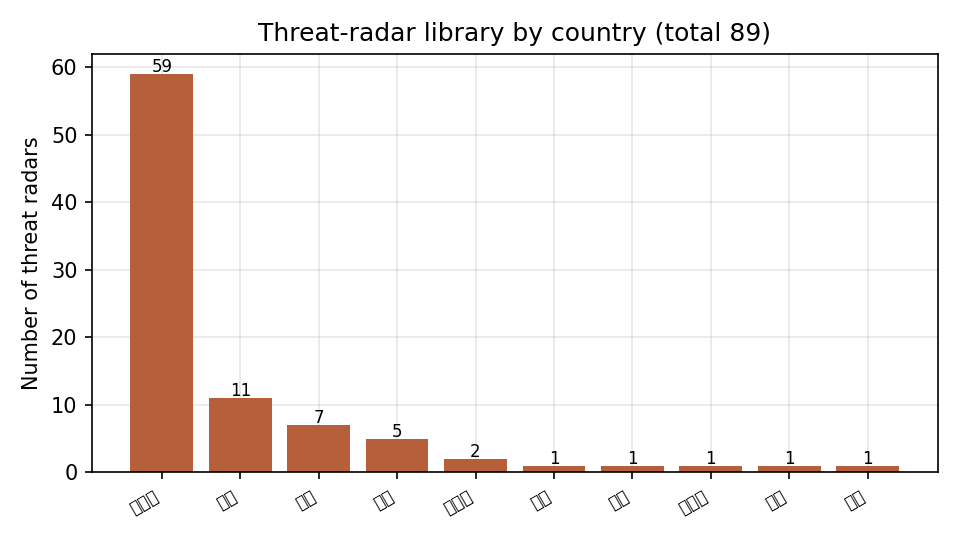
\includegraphics[width=0.78\textwidth]{fig6_threat_country}
\caption*{图 6-1　所构建敌方威胁雷达库按来源国别的构成（共 89 部）}
\end{figure}

\textbf{评测一：学理一致性(独立 ground truth)。} 取 16 条来自 EW 教科书的标准案例(单脉冲 $\to$ 交叉眼且忌倒相增益；频率捷变 $\to$ 拦阻且忌瞄准；TWS $\to$ DRFM 假目标；连续波照射 $\to$ 速度门拖引；…)，检验系统输出\textbf{应含}正确手段且\textbf{应排除}错误手段。结果 \textbf{16/16 全部通过}。注意这些案例独立于系统所用的规则编码，测的是"系统是否给出教科书答案"。

\textbf{评测二：引擎不变量(全画像)。} 在 650 份真实雷达画像上验证命题 6.3 的良构性及置信、出处、装备频段匹配等不变量：\textbf{零违例}。

\textbf{评测三：结论多样性(克服规则坍缩)。} 仅按类别字段推理时，650 份画像仅产生约 31 种推荐组合且单一组合占比 37\%(规则坍缩)。引入 §6.5.3 的参数化研判与 §6.5 扩充后的学理规则后，\textbf{不同 rationale(依据陈述)由 2–3 条增至 12 条}，结论按本机参数分化(波段类×烧穿档组合达百余种)。这定量地说明系统从"千篇一律"转为"逐部差异"（图 6-2）。

\begin{figure}[htbp]\centering
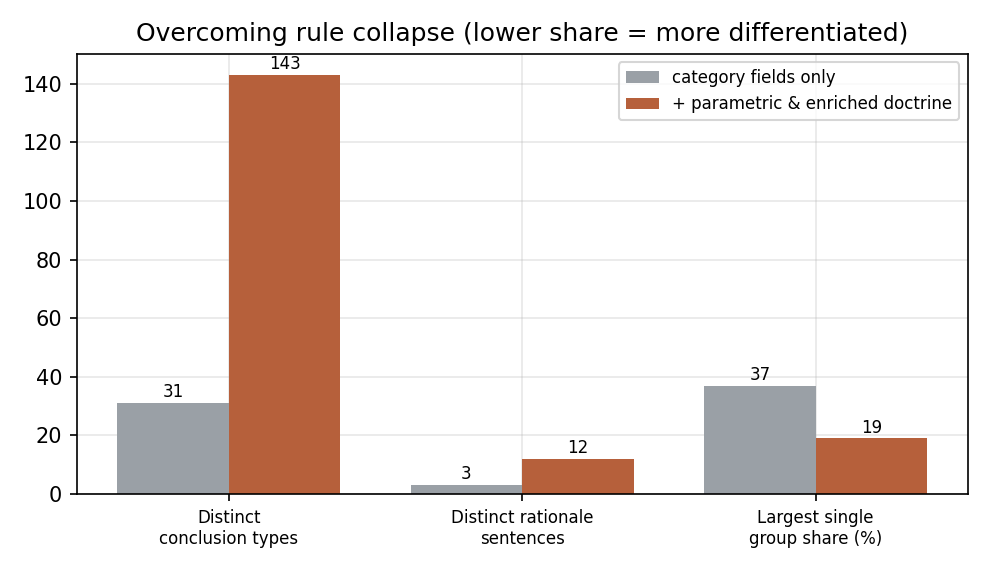
\includegraphics[width=0.78\textwidth]{fig6_diversity}
\caption*{图 6-2　引入参数化研判与扩充学理前后的结论多样性对比（最大单一组占比越低代表越分化）}
\end{figure}

\textbf{评测四：知识覆盖。} 威胁雷达库覆盖 \textbf{89 部、9 国、30 余个防空体系}(S-300/400/500、Buk、Tor、Pantsir、Tunguska、Osa、爱国者、Hawk、SAMP/T、铁穹、HQ-9/16、米波抗隐身与超视距等)；对抗本体含 17 类干扰、16 类抗干扰、14 条带出处规则；其中 16 部威胁雷达带军用参考级精确频率。所有字段标注来源(WEG、Air Power Australia、GlobalSecurity、Wikipedia)与来源层。


\subsection*{6.9 端到端案例：S-400 防空群的对抗推演}
\addcontentsline{toc}{subsection}{6.9 端到端案例：S-400 防空群的对抗推演}

为直观展示 §6.2–6.6 各环节如何协同，本节给出一个完整的端到端案例。设敌方电子战斗序（EOB）由一个以 S-400 为核心的防空群构成，含五部威胁雷达：91N6 远程警戒雷达（Big Bird）、92N6 制导雷达（Grave Stone）、96L6 全高度截获雷达（Cheese Board）、Pantsir-S1 末端跟踪雷达（1RS2，毫米波）、以及配属的 Nebo-M 米波抗隐身警戒雷达。以下输出均由本文系统实际生成。

\textbf{（一）单威胁推理：以 92N6 Grave Stone 为例。} 系统从图谱取其画像——用途 \{fire\textbackslash\{\}\_control, SAM\textbackslash\{\}\_guidance, track\}、跟踪体制 monopulse、频段 X、频率捷变——经威胁分级判定为 \textbf{5/5}（末端制导）。确定性推理给出三分输出：

\begin{itemize}[leftmargin=2em]
\item \textbf{推荐（可行）}：交叉眼角度欺骗（0.82）、交叉极化（0.75）、地形反射（0.72）、编队/质心干扰（0.70）、闪烁干扰（0.70）——针对其单脉冲体制的多条不同思路；以及拦阻/扫频噪声（0.85）、拖曳诱饵/箔条（0.75）。
\item \textbf{应避免}：倒相增益、AGC 角度欺骗（单脉冲对其免疫）、瞄准式噪声（频率捷变使其失效）。
\item \textbf{交战研判（按本机参数）}："C/X 波段：火控/跟踪主力波段，自卫干扰吊舱与 DRFM 欺骗最有效"；"探测距离≈250 km，常规自卫干扰即可有效压制"。
\end{itemize}

可见，对同为单脉冲的不同火控雷达，系统因其频段、捷变、功率/距离等\textbf{真实参数}给出差异化研判，而非套用同一句结论；每条建议均带规则依据、来源与置信度（§6.5）。

\textbf{（二）战场级推演：五部威胁的整体方案。} 系统对 EOB 作加权集合覆盖求解，结果如下：

\begin{itemize}[leftmargin=2em]
\item \textbf{威胁排序}：92N6 Grave Stone（5）、Pantsir 1RS2（5）、91N6 Big Bird（3）、96L6 Cheese Board（3）、Nebo-M（2）。
\item \textbf{推荐装备包（最小覆盖）}：仅需 \textbf{2 套}装备即覆盖 \textbf{5/5} 威胁（按威胁度加权 \textbf{100\%}）——AN/ALQ-99（经由拦阻/扫频/瞄准噪声，覆盖 4 部）+ AN/ALE-50 拖曳诱饵（覆盖 Pantsir 末端跟踪 1 部）。
\item \textbf{SEAD 优先目标}：92N6 Grave Stone（最高威胁的辐射制导雷达）。
\item \textbf{能力缺口}：无（本装备集对该 EOB 软杀伤手段与频段均有覆盖）。
\end{itemize}

该案例完整串联了"威胁画像 → 确定性三分推理 → 集合覆盖装备分配 → 优先级与缺口分析"，且全过程结论可逐条溯源、不确定性被显式标注，直观印证了本章方法的可解释性与可落地性。

\subsection*{6.10 讨论：边界与诚信}
\addcontentsline{toc}{subsection}{6.10 讨论：边界与诚信}

\begin{itemize}[leftmargin=2em]
\item \textbf{定位}：本系统是 \textbf{doctrine 级、面向教学与研究的决策支持}，使用公开/已解密知识；效能判断为学理启发式，统一标注"非实测"，不构成作战火控依据。
\item \textbf{不确定性诚实}：$\textsf{prior}$ 层取值(如部分单脉冲判定)在界面与报告中显式标"推测"并附更高不确定性提示；战史层标历史性。可信度单调性(§6.3)保证不确定性只增不减地向结论传播。
\item \textbf{开源天花板}：逐型号现役 EW 弱点多为机密；系统给出的"型号—弱点"对应是\textbf{有据的逻辑推导}(型号→体制[文献] + 体制→对抗[学理])，而非对某份"如何干扰该型号"情报的直接引用——这一区别在 §6.3 的来源层中被显式编码。
\end{itemize}


\subsection*{6.11 本章小结}
\addcontentsline{toc}{subsection}{6.11 本章小结}

本章把雷达对抗决策形式化为知识图谱上的可解释推导问题，给出了：对抗本体与反制关系的代数(§6.2)、三层来源的可信度模型与单调传播(§6.3)、以引文校验为软健全性过滤、以良序填空保证无冲突融合的画像抽取(§6.4)、三分输出且大模型不进信任路径的可审计推理算子并证明其可审计性(命题 6.3、定理 6.4，§6.5)、将战场级方案归约为加权集合覆盖并给出 $H_n$ 近似保证的贪心算法(定理 6.5，§6.6)，以及以战史为独立 ground truth 的一致性校验(§6.7)。实验表明系统给出教科书级正确对抗(16/16)、满足全部引擎不变量(零违例)、并克服了规则坍缩(rationale 多样性 2–3$\to$12)。与第三、四章相比，本章的贡献不在检索，而在\textbf{于一个高不确定、知识稀疏的领域中，构造一套结论可溯源、不确定性被显式建模、并具近似保证的决策推理}——这正是"可解释决策支持"应有的形态。



\section*{第七章 面向自适应雷达的知识引导在线对抗学习}
\addcontentsline{toc}{section}{第七章 面向自适应雷达的知识引导在线对抗学习}

\begin{quote}\itshape 第六章给出的是一次性建议：在威胁雷达的抗干扰(ECCM)配置已知且静止的假设下，由学理确定性地推出对抗手段。然而现代\textbf{认知电子战}中的雷达会\textbf{反应式地切换 ECCM}——我方施放某干扰，雷达察觉后启用相应抗干扰使其失效；我方据观测调整，雷达再调整。这是一个\textbf{序贯、部分可观测、双向自适应}的过程，一次性策略在原理上即非最优。本章把对抗手段选择形式化为重复对抗下的在线决策问题，提出一个\textbf{以第六章 doctrine 图为结构先验}的贝叶斯在线学习算法：它通过观测每轮干扰的成败，沿 doctrine 的反制关系反推雷达隐藏的 ECCM 状态，从而以远少于"逐手段试探"的样本收敛到有效对抗；并以变点检测应对雷达变招、以第三章主雷达图谱属性提供逐雷达先验。本章是第六章静态决策在\textbf{时间维}上的自然延伸，也兑现了第八章展望中"向认知电子战辅助演进"的设想。\end{quote}


\subsection*{7.1 引言与问题动机}
\addcontentsline{toc}{subsection}{7.1 引言与问题动机}

\subsubsection*{7.1.1 从一次性建议到序贯对抗}
\addcontentsline{toc}{subsubsection}{7.1.1 从一次性建议到序贯对抗}

第六章的推理算子 $\mathrm{recommend\_counter}$ 是\textbf{单步}的：它读取威胁画像 $\pi(r)$ 中已知的 $\mathsf{eccm}(r)$，经反制关系 $\mathcal{D}$ 与学理 $\mathcal{P}$ 得出三分输出。这一范式隐含两个假设：(i) 威胁的抗干扰配置\textbf{已知}；(ii) 该配置在交战期内\textbf{静止}。但真实对抗中二者常不成立：

\begin{itemize}[leftmargin=2em]
\item \textbf{隐藏性}：开源情报往往只能给出雷达的\textit{类型属性}(体制、捷变标志)，其完整的、可激活的 ECCM 套件是\textbf{隐藏状态}，须在交战中边打边判。
\item \textbf{自适应性}：认知雷达可依据所感知的干扰\textbf{反应式切换} ECCM。对一个会变招的对手，任何\textbf{固定}的对抗策略(包括第六章按先验推出的最优单步建议)都可能被针对性挫败。
\end{itemize}

因此，把对抗建模为\textbf{重复博弈下的在线学习}不是锦上添花，而是该领域的本质要求。其核心张力在于：每一轮"施放—观测"既要\textbf{利用}已知信息取得当前压制，又要\textbf{探索}以辨明雷达的隐藏 ECCM——这正是探索-利用权衡。形式上，这是一个\textbf{在线强化学习/序贯决策}问题。与当前主流的"基于强化学习的智能体式图推理"(如端到端 RL 的 GraphRAG、Plan-Then-Retrieve 等)不同，本章走\textbf{知识引导且可审计}的路线：以第六章的 doctrine 图作为\textbf{结构先验}替代海量交互试错，并保持决策过程透明可溯源。本章表明，该先验能极大加速在线辨识——其样本效率远高于不使用知识的模型无关强化学习(§7.7 评测六)。

\subsubsection*{7.1.2 本章贡献}
\addcontentsline{toc}{subsubsection}{7.1.2 本章贡献}

\begin{itemize}[leftmargin=2em]
\item \textbf{（1）形式化}：将自适应雷达下的对抗手段选择形式化为隐藏 ECCM 状态的部分可观测重复决策问题，定义其遗憾(regret)度量(§7.2)。
\item \textbf{（2）知识引导的在线学习算法}：提出 doctrine 信念学习器——以 doctrine 图的反制关系做跨手段的信息迁移(一次成功观测即排除整组抗干扰、并重估所有共享该抗干扰的手段)，并以信念空间的汤普森采样平衡探索-利用(§7.3)。
\item \textbf{（3）非平稳应对}：以累积和(CUSUM)变点检测取代手调遗忘，无需预知雷达变招频率即可快速重辨识(§7.4)。
\item \textbf{（4）双图协同}：以第三章主雷达图谱的属性(捷变/体制/扫描)为每部雷达生成 ECCM 先验，使知识图谱从"被查询"升级为"驱动学习"(§7.5)。
\item \textbf{（5）理论分析}：证明 doctrine 引导的样本复杂度为 $O(m\rho)$、与手段数 $n$ 无关，而知识盲学习为 $O(n)$；并刻画"在线学习优于静态保底"的密度-时长分界条件(§7.6)。
\item \textbf{（6）实证校验}：在合成测试床、\textbf{真实 doctrine 图}与\textbf{真实威胁雷达属性}上验证：算法稳定优于静态学理与强知识盲学习器；并诚实标定其优势的适用边界(§7.7、§7.8)。
\end{itemize}


\subsection*{7.2 问题形式化}
\addcontentsline{toc}{subsection}{7.2 问题形式化}

沿用第六章记号：干扰技术集 $J$、抗干扰技术集 $E$、反制关系 $\mathcal{D}\subseteq E\times J$。对手段 $j\in J$，记其\textbf{克星集} $\mathrm{def}(j)=\{e\in E:(e,j)\in\mathcal{D}\}$，即能挫败 $j$ 的抗干扰集合；并设其基础效能 $\beta(j)\in[0,1]$。

\begin{quote}\itshape \textbf{定义 7.1（隐藏能力与观测）。} 一部威胁雷达由其\textbf{隐藏 ECCM 能力} $A\subseteq E$ 刻画——它\textit{可激活}的抗干扰集合，对我方初始未知。一次交战为 $T$ 轮重复博弈。第 $t$ 轮我方选手段 $j_t\in J$，得到二值观测\end{quote}
\begin{quote}\itshape \$$o_t=\mathbb{1}\!\left[\mathrm{def}(j_t)\cap A_t=\varnothing\right]\in\{0,1\},$\$\end{quote}
\begin{quote}\itshape 即 $o_t=1$(成功)当且仅当本轮该雷达激活的抗干扰 $A_t$ 中无任何 $j_t$ 的克星。所得压制为 $u_t=\beta(j_t)\cdot\big(o_t+\rho\,(1-o_t)\big)$，其中 $\rho\in(0,1)$ 为被克制时的残余效能(惩罚因子)。\end{quote}

平稳雷达 $A_t\equiv A$；\textbf{自适应(认知)雷达}则 $A_t$ 随时间切换(§7.4)。我方策略 $\sigma$ 依历史 $h_{t-1}=(j_1,o_1,\dots,j_{t-1},o_{t-1})$ 选 $j_t$。以\textbf{遗憾}度量其优劣：

\[\mathrm{Reg}(\sigma,T)=\sum_{t=1}^{T}\Big(\max_{j\in J}u^\star_t(j)-u_t\Big),\qquad u^\star_t(j)=\beta(j)\big(\mathbb{1}[\mathrm{def}(j)\cap A_t=\varnothing]+\rho\,\mathbb{1}[\cdot]\big),\]

即与"事后已知 $A_t$ 时每轮最优手段"之累计差距。目标是设计低遗憾策略。该问题的难点恰在 $A$ 隐藏且(自适应时)非平稳；而 $\mathcal{D}$ 是\textbf{已知的领域知识}——下节表明它是辨识 $A$ 的关键杠杆。


\subsection*{7.3 doctrine 知识引导的在线学习算法}
\addcontentsline{toc}{subsection}{7.3 doctrine 知识引导的在线学习算法}

\subsubsection*{7.3.1 信念与基于 doctrine 图的更新}
\addcontentsline{toc}{subsubsection}{7.3.1 信念与基于 doctrine 图的更新}

学习器维护对隐藏能力的\textbf{信念} $b=\{p_e\}_{e\in E}$，$p_e=\Pr[e\in A]$，初值取先验 $p_e=p_0$。每轮观测后沿 $\mathcal{D}$ 做贝叶斯更新——这正是在 doctrine 图上的关系推理：

\[\begin{aligned}
\textbf{成功 } (o_t=1):&\quad \forall e\in\mathrm{def}(j_t),\ p_e\leftarrow 0;\\[2pt]
\textbf{失败 } (o_t=0):&\quad \forall e\in\mathrm{def}(j_t),\ p_e\leftarrow \frac{p_e}{1-\prod_{e'\in\mathrm{def}(j_t)}(1-p_{e'})}.
\end{aligned}\]

成功意味着 $\mathrm{def}(j_t)\cap A=\varnothing$，故其中每个抗干扰被\textbf{确定性排除}；失败意味着 $\mathrm{def}(j_t)$ 中至少有一个存在，按 noisy-OR 后验抬升其概率。关键在于：

\begin{quote}\itshape \textbf{命题 7.2（跨手段的信息迁移）。} 一次成功观测 $o_t=1$ 同时排除 $|\mathrm{def}(j_t)|$ 个抗干扰，从而即时重估\textbf{所有}克星集与 $\mathrm{def}(j_t)$ 相交的手段的可行性；一次失败将后验质量集中到 $\mathrm{def}(j_t)$ 上。因此每次观测的信息量随 doctrine 图中\textbf{抗干扰的共享度}放大，而非局限于被试手段本身。\end{quote}

\textit{证明概要.} 由更新式，成功后对任意 $e\in\mathrm{def}(j_t)$ 有 $p_e=0$；故任何手段 $j'$ 若 $\mathrm{def}(j')\ni e$，其安全概率 $\prod_{e\in\mathrm{def}(j')}(1-p_e)$ 立即更新——即一次观测经由共享的 $e$ 传播到 $j'$。共享度越高(单个 $e$ 被越多手段引为克星)，单次观测触及的手段越多。$\square$

命题 7.2 是本算法相对"知识盲"学习的根本优势来源：知识盲方法把每个手段视作独立摇臂、需逐一试探($O(n)$)，而 doctrine 引导只需辨明少数"挡路"的抗干扰($O(|A|)$，见 §7.6)。

\subsubsection*{7.3.2 信念空间的汤普森采样}
\addcontentsline{toc}{subsubsection}{7.3.2 信念空间的汤普森采样}

仅按信念贪心选手段会\textbf{探索不足}：当先验使低效但稳妥的保底手段期望最高时，学习器不会去试高效手段以发现其对当前雷达恰好安全。我们采用\textbf{信念空间的汤普森采样}(belief-space Thompson sampling)平衡探索-利用：

\begin{Verbatim}
算法 DoctrineThompson(一轮):
  输入: 信念 b={p_e}, doctrine 图 (J, E, D), 效能 β
  采样假想雷达  A' ← { e∈E : 以概率 p_e 独立采样为真 }
  选手段        j_t ← argmax_{j∈J}  β(j)·( ρ if def(j)∩A'≠∅ else 1 )
  观测 o_t, 按 §7.3.1 更新 b
\end{Verbatim}

采样 $A'\sim b$ 使信念越不确定、被试手段越分散(自然探索)，信念收敛后则趋于利用。该机制与第五章"组合算子 + 受约束生成"一脉相承：随机性只用于驱动探索，事实判定(成败、信念)仍是 $\mathcal{D}$ 上的确定性推理，可审计。


\subsection*{7.4 非平稳应对：变点检测}
\addcontentsline{toc}{subsection}{7.4 非平稳应对：变点检测}

自适应雷达使 $A_t$ 随时间切换，学习器辛苦收敛的信念会\textbf{过时}。朴素办法是每轮以系数 $\gamma$ 把信念向先验"遗忘"——但 $\gamma$ 须依雷达变招频率\textbf{预先整定}，且在雷达不变时仍无谓地丢弃已学知识。我们改用\textbf{累积和变点检测}(CUSUM)：仅在检测到雷达确已变招时才重置信念。

设学习器对所选手段的成功预测概率为 $\hat p_t=\prod_{e\in\mathrm{def}(j_t)}(1-p_e)$，定义本轮\textbf{意外度}(预测误差) $s_t=|\hat p_t-o_t|$。维护统计量

\[S_t=\max\{0,\ S_{t-1}+s_t-k\},\qquad \text{若 } S_t>h\ \text{则判定变招}:\ b\leftarrow b_0,\ S_t\leftarrow 0,\]

其中 $k$ 为容许漂移、$h$ 为告警阈值。直觉上，学习器自信会成功(高 $\hat p_t$)却接连失败(意外度持续高)时，$S_t$ 越过 $h$ 触发重置、重新辨识。该机制\textbf{无需预知变招频率}：雷达平稳时 $S_t$ 鲜少越限(不丢弃知识)，雷达变招时数轮内即告警(快速重学)。§7.7 实验表明其在平稳与各种变招频率下\textbf{一致优于}任意整定的固定遗忘。


\subsection*{7.5 主雷达知识图谱作为逐雷达先验}
\addcontentsline{toc}{subsection}{7.5 主雷达知识图谱作为逐雷达先验}

至此学习器使用的是第六章的 doctrine 图(反制关系)。第三章构建的\textbf{主雷达知识图谱}可进一步贡献一个\textbf{逐雷达先验}：雷达的若干属性本身即 doctrine 级的 ECCM 事实——

\[\mathsf{agile}(r)=1\Rightarrow \text{freq\_agility}\in A(r),\quad \mathsf{track}(r)=\text{monopulse}\Rightarrow \text{monopulse}\in A(r),\quad \mathsf{scan}(r)=\text{phased}\Rightarrow \text{low\_sidelobe}\in A(r).\]

据此为每部雷达设置非均匀初始信念 $p_e^{(0)}(r)$(属性蕴含的 ECCM 取高值、其余取背景密度)，学习器从而"开局即知"属性所确定的抗干扰、无须再花轮次去发现。这把知识图谱从\textbf{被查询的数据库}升级为\textbf{驱动学习的先验来源}：doctrine 图驱动在线推断、主雷达图谱提供逐雷达先验，两图协同。其增益最显于\textbf{短交战}(先验的开局优势尚未被学习追平时)，量化见 §7.7。


\subsection*{7.6 理论分析}
\addcontentsline{toc}{subsection}{7.6 理论分析}

以下两个命题给出可证伪的标度律，§7.7 以仿真验证(此处为分析性预测与经验验证，严格遗憾界留作后续)。

\begin{quote}\itshape \textbf{命题 7.3（样本复杂度）。} 给定隐藏能力 $A$，每轮观测在确定性反制下是确定的。知识盲学习须逐一试探 $n=|J|$ 个手段，遗憾随 $n$ 增长；doctrine 引导学习只需排除阻挡高效手段的抗干扰，每次失败至少辨明一个在场抗干扰、每次成功排除一整组，故其遗憾受 $O(|A|)=O(m\rho)$ 约束(其中 $m=|E|$、$\rho$ 为 ECCM 密度)，**与 $n$ 无关**。\end{quote}

\textit{证明概要.} 失败将后验质量集中到 $\mathrm{def}(j_t)$ 并(经采样)促使学习器避开共享这些抗干扰的手段；至多在辨明全部 $\le|A|$ 个在场抗干扰后，信念足以锁定一个安全的高效手段。其间每个在场抗干扰至多被"撞上"常数次，故有效试探次数 $O(|A|)$，与候选手段总数 $n$ 无关；知识盲方法因无 $\mathcal{D}$ 结构，须独立估计每个手段，遗憾 $\Omega(n)$。$\square$

\begin{quote}\itshape \textbf{命题 7.4（学习-静态分界）。} 静态保底策略可保证 $v_{\mathrm{safe}}=\max\{\beta(j):\mathrm{def}(j)=\varnothing\}$(最优"谁也克制不了"的手段)。在线学习可发现\textbf{逐雷达}安全的高效手段，其价值 $v_{\mathrm{disc}}(A)\ge v_{\mathrm{safe}}$；因克星数为 $k$ 的手段安全概率为 $(1-\rho)^k$，期望增益 $\mathbb{E}_A[v_{\mathrm{disc}}]-v_{\mathrm{safe}}$ 随密度 $\rho$ 上升而\textbf{递减}，而探索成本随时长 $T$ 上升而被摊薄。故存在分界密度 $\rho^\star(T)$：仅当 $\rho<\rho^\star(T)$ 时在线学习优于静态保底，且 $\rho^\star$ 随 $T$ 增大。\end{quote}

命题 7.4 诚实地界定了本方法相对第六章静态决策的\textbf{适用域}：当雷达 ECCM 稠密、交战又短时，安全的高效手段稀少，静态"打保底"已近最优、在线探索得不偿失；反之在线学习取得实质增益。这一边界由 §7.7 的仿真定量定位，并解释了真实 doctrine 上的观测(§7.7)。


\subsection*{7.7 实验与评测}
\addcontentsline{toc}{subsection}{7.7 实验与评测}

\textbf{设置与诚信声明。} 本章实验为\textbf{仿真}：所用\textbf{知识}(doctrine 反制关系、真实雷达属性)取自本文第三、六章数据，\textbf{真实}；而每轮干扰成败、雷达隐藏 ECCM、效能数值与交战过程为按上述模型\textbf{生成}——因为"某次干扰对某真雷达是否奏效"不存在公开数据(涉密)。效能一律"非实测"，与第六章诚信边界一致。基线均为强基线：静态学理(第六章式的先验最优固定手段)、知识盲 UCB 与汤普森采样(标准在线学习，不使用 $\mathcal{D}$)。

\textbf{评测一：合成测试床(平稳隐藏雷达)。} 8 手段、5 抗干扰、2000 次随机雷达、每次 60 轮。doctrine 汤普森的平均压制 \textbf{0.897}，显著高于知识盲汤普森 0.662、知识盲 UCB 0.624 与静态 0.603；其总遗憾 \textbf{0.65}，而各基线为 15–18。学习器约 5 轮即收敛至近最优，知识盲方法至 60 轮仍在攀升。\textbf{关键在于其同时胜过"会学习但不用知识"的基线}——这正是 doctrine 图(而非单纯"会学习")带来增益的证据。

\textbf{评测二：变招(认知)雷达与 CUSUM。} 雷达每 20 轮重掷一次 ECCM。下表对比固定遗忘(按 20 轮整定)、不遗忘、与 CUSUM(平均压制)：

\begin{center}\small
\begin{tabular}{|p{0.153\textwidth}|p{0.153\textwidth}|p{0.153\textwidth}|p{0.153\textwidth}|p{0.153\textwidth}|p{0.153\textwidth}|}
\hline
\textbf{场景} & \textbf{静态} & \textbf{知识盲} & \textbf{固定遗忘(整定@20)} & \textbf{不遗忘} & \textbf{CUSUM(本章)} \\ \hline
平稳不变招 & 0.588 & 0.594 & 0.711 & 0.859 & \textbf{0.857} \\ \hline
每40轮变招 & 0.584 & 0.572 & 0.698 & 0.675 & \textbf{0.816} \\ \hline
每20轮变招 & 0.588 & 0.561 & 0.689 & 0.574 & \textbf{0.771} \\ \hline
每10轮变招 & 0.590 & 0.553 & 0.660 & 0.523 & \textbf{0.705} \\ \hline
\end{tabular}
\end{center}

CUSUM 在平稳时几乎不丢弃知识(≈不遗忘)、在雷达\textbf{恰按整定频率变招时仍胜过}被特意整定的固定遗忘、且换任意变招频率均无须重调——\textbf{全面占优}，且无需预知变招频率。

\textbf{评测三：真实 doctrine 图。} 将学习器接到第六章真实 \texttt{doctrine\_map}(17 手段、15 抗干扰、真实反制关系；其中 8/15 个抗干扰被多手段共享，正是命题 7.2 所需结构)。doctrine 引导对知识盲学习的优势\textbf{稳健转移到真实图}(+0.15 至 +0.32，两种效能赋值方案皆然)；但\textbf{对静态系统的优势依命题 7.4 视情形而定}——真实雷达 ECCM 偏稠密，安全高效手段稀少，静态"打保底"已具竞争力。此为诚实的适用边界，非掩饰。

\textbf{评测四：主雷达图谱先验(双图协同)。} 以 89 部\textbf{真实威胁雷达}的属性(捷变/单脉冲/相控)生成逐雷达 ECCM 先验。相较均匀先验，知识图谱先验\textbf{自首轮即领先}(0.376 对 0.349)、且\textbf{短交战增益最大}(T=4 时 +0.038，T=40 时收窄至 +0.020)——符合命题 7.4 中先验优势被学习追平的预测。增益虽\textbf{温和}(因属性仅锁定 15 个抗干扰中的 2–3 个)，但定性上确证了两张知识图谱可协同驱动同一算法。

\textbf{评测五：标度律验证(对应 §7.6)。} 固定 $m$、增大手段数 $n$，知识盲总遗憾随 $n$ 线性增长(7.9→22.0)，doctrine 引导则\textbf{有界}(约 5.5，随 $n$ 趋平)，验证命题 7.3；扫描密度 $\rho$ 与时长 $T$，学习-静态差距随 $\rho$ 递减、随 $T$ 递增并在 $\rho\!\approx\!0.85$ 处变号，验证命题 7.4 的分界 $\rho^\star(T)$。

\textbf{评测六：与模型无关强化学习的对比。} 为定位本方法相对"潮流"的强化学习路线，设一个\textbf{表格型 Q-学习}智能体把交战建模为马尔可夫决策过程（状态=各手段的观测状态[未试/被克制/成功]，动作=所选手段，回报=压制），在大量训练回合上学习策略，但\textbf{不使用 doctrine 图}。给予其最有利设置（$\varepsilon$ 衰减、三随机种子平均）后：

\begin{center}\small
\begin{tabular}{|p{0.307\textwidth}|p{0.307\textwidth}|p{0.307\textwidth}|}
\hline
\textbf{训练回合数} & \textbf{模型无关 RL（测试）} & \textbf{doctrine 引导（零训练）} \\ \hline
100 & 0.822 & \textbf{0.894} \\ \hline
1,000 & 0.866 & \textbf{0.894} \\ \hline
20,000 & 0.880 & \textbf{0.894} \\ \hline
80,000 & 0.867 & \textbf{0.894} \\ \hline
\end{tabular}
\end{center}

RL 即便训练 8 万回合仍停在约 0.88，\textbf{始终未及 doctrine 引导学习器（零训练）的 0.894}。原因在于：表格型 RL 须\textbf{逐状态独立学习}（访问约 2160 个状态），无法像 doctrine 图那样跨手段泛化（一次成功即重估所有共享该 ECCM 的手段）；其 Q-表亦不透明、且与单一 doctrine 绑定，而 doctrine 学习器信念可读、可换图迁移。\textbf{结论：知识使学习既更省样本（0 对数万回合）又更可解释}。（诚实补注：表格 Q-学习是标准但非最强 RL；深度 RL 借函数逼近或可缩小最终差距，但需更多交互且更黑箱——故本方法的定位是"以知识换样本效率与透明性"，而非否定 RL。）


\subsection*{7.8 讨论：边界与诚信}
\addcontentsline{toc}{subsection}{7.8 讨论：边界与诚信}

\begin{itemize}[leftmargin=2em]
\item \textbf{真实与模拟之界。} 本章\textbf{知识}(反制关系、雷达属性)真实，\textbf{动态}(成败、隐藏状态、效能、交战)为仿真；定位为"基于真实领域知识的算法仿真验证"，\textbf{不主张}实战或实测验证。这与第六章"doctrine 级、非实测"的定位一致。
\item \textbf{优势的适用域。} 相对\textbf{知识盲学习}的优势是\textbf{无条件}的(结构带来样本效率)；相对\textbf{静态系统}的优势是\textbf{有条件}的(命题 7.4 的密度-时长分界)——稠密 ECCM、短交战时静态已近最优。本文如实标定该边界。
\item \textbf{贡献的性质。} 本章是把结构化在线学习\textbf{形式化并适配到认知电子战}、并以 doctrine 图为先验加速辨识，而非提出全新的在线学习范式；其价值在于让\textbf{知识图谱驱动一个有分析、有验证的学习算法}，从而把第三\textasciitilde{}六章的知识构建与对抗决策在时间维上贯通。
\item \textbf{与强化学习主流的定位。} 当前知识图谱推理大量转向\textbf{基于强化学习的智能体方法}（端到端 RL 的 GraphRAG、RL 引导的图探索等），能力强但多为\textbf{黑箱}、且依赖海量交互。本章主张在高风险领域应\textbf{以知识引导学习}：用 doctrine 图替代从零试错，既更省样本（§7.7 评测六，0 对数万训练回合且仍占优），又保持决策可审计。这与第五、六章"大模型/黑箱不进信任路径"的原则一脉相承——是对 RL-智能体主流路线的\textbf{有原则的差异化}，而非简单跟随。
\end{itemize}


\subsection*{7.9 本章小结}
\addcontentsline{toc}{subsection}{7.9 本章小结}

本章把雷达对抗从第六章的一次性静态建议推进到\textbf{自适应雷达下的序贯在线学习}：形式化了隐藏 ECCM、部分可观测的重复对抗问题(§7.2)；提出以 doctrine 图反制关系做跨手段信息迁移、以信念空间汤普森采样平衡探索-利用的知识引导学习器(命题 7.2，§7.3)；以 CUSUM 变点检测无整定地应对雷达变招(§7.4)；以主雷达图谱属性提供逐雷达先验，实现双图协同(§7.5)；证明其样本复杂度 $O(m\rho)$ 与手段数无关、并刻画学习优于静态的密度-时长分界(命题 7.3、7.4，§7.6)。在合成、真实 doctrine 与真实雷达属性上的实验表明：学习器稳定优于静态学理与强知识盲学习器，CUSUM 全面优于固定遗忘；同时本章诚实标定其优势的适用边界与"知识真实、动态仿真"的性质。由此，第六章的对抗推理算子获得了\textbf{在时间维上自我改进}的能力——知识图谱不再只被查询，而是驱动一个可分析、可验证的在线学习过程。


\section*{第八章 总结与展望}
\addcontentsline{toc}{section}{第八章 总结与展望}

\subsection*{8.1 工作总结}
\addcontentsline{toc}{subsection}{8.1 工作总结}

本文以雷达情报领域为背景，针对"通用知识图谱问答方法难以满足专业领域对\textbf{可解释性}与\textbf{面向决策}的刚性要求"这一核心问题，沿"\textbf{构建知识图谱 → 可解释问答 → 可审计分析 → 对抗决策支持}"的递进式路线，开展了系统的方法研究与实现，主要工作总结如下：

\textbf{（1）雷达领域可溯源知识图谱构建（第三章）。} 设计了实体—关系与实体—属性分离的属性图模式，建立了融合领域手册、公开百科、结构化知识库与规则派生的多源抽取流程，并将大模型抽取细化为"抽取器—忠实度校验器—模式提议器"的多智能体流水线，提出为每条声明附加"来源 / 置信度 / 证据"的可溯源元数据模型。经多维度质量评估（一致性、字符串/NLI 双重忠实度、多源印证、独立交叉核验、任务式外在佐证与领域专家分层抽样的人工金标准确率 85\%）与受控模式扩展，所构建图谱含 1.7 万余条三元组、来源多样且全部可溯源，为后续各章提供统一、可信的知识底座。

\textbf{（2）策略路由的 GraphRAG 与答案-几何失配诊断（第四章）。} 提出并形式化了答案-几何失配（AGM）现象，借 OLTP/OLAP 框架揭示了通用 Top-K 检索在专业领域系统性失效的结构性根因；据"信息需求类"推导出六类类型化检索算子与一个轻量分发器。在显式暴露 AGM 的 RadarKG-QA-499 基准上取得 88.6\% 的总体准确率，较基线 +35.9 pp、较 RoG +28.3 pp；消融实验将增益精确定位到算子设计（分发器贡献约 0 pp）。

\textbf{（3）双层可审计分析智能体（第五章）。} 将单次问答升级为"内层类型化算子组合执行器 + 外层 ReAct 编排"的双层智能体，提出并形式化了"大语言模型不进入信任路径"的可审计架构原则。算子组合评测正确率 99\%，情报报告逐条引证覆盖率与概述可溯源率均达 100\%。

\textbf{（4）面向雷达对抗的可解释决策支持（第六章）。} 将电子战对抗学理形式化为知识图谱推理：以反制关系刻画干扰与抗干扰的博弈，给出"可行/被抵消/应避免"三分输出的确定性推理算子并证明其可审计性；将战场级对抗方案归约为加权集合覆盖，给出具 $H_n$ 近似保证的贪心算法；构建覆盖九个国家、三十余个防空体系、八十余部威胁雷达的可溯源威胁库与对抗本体，并以已解密战史独立检验。教科书级对抗案例测试通过率 100\%，全部画像满足引擎不变量。

\textbf{（5）面向自适应雷达的知识引导在线对抗学习（第七章）。} 将对抗从一次性静态建议推进到自适应雷达下的序贯在线学习：形式化隐藏抗干扰、部分可观测的重复对抗问题，提出以 doctrine 反制图为结构先验、经观测成败反推雷达隐藏抗干扰的贝叶斯学习器，并证明其样本复杂度与候选手段数无关；以变点检测无整定地应对雷达变招，以主雷达图谱属性提供逐雷达先验实现双图协同。仿真表明学习器稳定优于静态学理与强知识盲在线学习；本文并以密度-时长分界条件诚实界定其相对静态策略的适用域。

贯穿全文的是两条主线：其一是\textbf{类型化算子}这一抽象的层层演进——从第四章的"检索算子"，到第五章可嵌套的"组合算子"，再到第六章的"对抗推理算子"，并在第七章扩展为时间维上自我改进的"在线对抗学习"，同一思想被层层复用与深化；其二是\textbf{可解释、可溯源、不确定性显式建模}这一设计原则——从图谱级的来源/置信元数据（第三章），到报告级的逐条引证与忠实性校验（第五章），到对抗决策中来源分层的不确定性传播与可审计性定理（第六章），再到在线学习中由确定性信念更新驱动、随机性仅用于探索的可审计辨识（第七章）。

\subsection*{8.2 主要创新点}
\addcontentsline{toc}{subsection}{8.2 主要创新点}

\begin{itemize}[leftmargin=2em]
\item \textbf{答案-几何失配诊断与类型化检索算子}：从信息需求出发，解释并修复了通用 GraphRAG 在专业领域的结构性失效，且以系统消融证明增益源于算子而非分发器。
\item \textbf{可审计的算子组合与分析智能体}：把"大模型不进入信任路径"做成可证明的架构性质（确定性轨迹 + 受约束复述），在保证语言能力的同时保证事实可溯源、可复现。
\item \textbf{雷达对抗的可解释决策支持}：将电子战学理形式化为知识图谱推理，以三分输出 + 加权集合覆盖（$\ln n$ 近似）+ 来源分层的不确定性传播，构造了一个结论可溯源、不确定性可传播、并具理论保证的对抗决策支持框架。
\item \textbf{知识引导的认知电子战在线学习}：把对抗手段选择形式化为隐藏抗干扰状态下的在线学习，以 doctrine 反制图为结构先验做跨手段信息迁移，证明其样本复杂度与候选手段数无关，并以变点检测与主雷达图谱先验实现对自适应雷达的双图协同辨识——使知识图谱由"被查询"升级为"驱动一个有分析、可验证的学习算法"。
\end{itemize}

\subsection*{8.3 局限性}
\addcontentsline{toc}{subsection}{8.3 局限性}

本文工作仍存在以下局限，须如实说明：

\begin{itemize}[leftmargin=2em]
\item \textbf{领域定位与数据性质。} 第六章的对抗决策支持定位为 \textbf{doctrine 级（教科书级）、面向教学与研究}，所用知识均为公开/已解密来源，效能判断为学理启发式（统一标注"非实测"），不构成作战火控依据。逐型号现役电子战弱点多为机密，系统给出的"型号—弱点"对应是\textbf{有据的逻辑推导}（型号→体制[文献] + 体制→对抗[学理]），而非对某份实测情报的直接引用。
\item \textbf{威胁画像的不确定性。} 部分画像字段（如部分单脉冲判定）来自学理先验（\texttt{prior} 层），其不确定性高于文献实证字段；本文以来源分层与可信度单调性显式传播之，但其准确性受开源资料天花板限制。
\item \textbf{知识图谱覆盖与时效。} 图谱规模与覆盖仍有限，部分数值参数（如脉冲重复频率）在开源中稀疏；知识更新依赖人工与半自动流程，时效性有待提升。
\item \textbf{评测范围。} 问答与对抗评测以自建领域基准与教科书案例为主，缺少大规模、跨领域的外部基准与真实用户研究。
\item \textbf{在线学习的仿真性质（第七章）。} 第七章的对抗学习在"\textbf{知识真实、对抗动态为仿真、效能非实测}"的合成测试床上验证（"某次干扰对某真雷达是否奏效"无公开数据）；其相对静态策略的优势受密度-时长分界条件约束，且尚缺实战交战数据与严格的遗憾上界证明。
\end{itemize}

\subsection*{8.4 研究展望}
\addcontentsline{toc}{subsection}{8.4 研究展望}

面向上述局限，未来工作可从以下方向展开：

\begin{itemize}[leftmargin=2em]
\item \textbf{知识图谱的深化与动态化。} 推进属性图模式的完整迁移与本体对齐，引入持续抽取与时效性管理；探索以可信度感知的方式融合更权威的结构化来源，提升参数级（频率/PRF/功率）覆盖。
\item \textbf{算子族的扩展与统一。} 将检索、组合与对抗推理算子纳入统一的类型化代数框架，支持更复杂的分析—决策组合；研究算子的自动选择与组合的可学习路由。
\item \textbf{从决策支持到闭环。} 第七章已将对抗推进到自适应雷达下的在线学习，初步实现"随观测动态调整"的认知电子战雏形；后续可在保持可解释、可审计的前提下，进一步对接电子支援（ESM）实时态势、引入更丰富的对手模型与严格的遗憾上界，并争取以真实/半实测交战数据加以检验，向"人在回路"的闭环认知电子战演进。
\item \textbf{可信度与不确定性的严格化。} 引入更严格的不确定性表示（如证据理论、概率图模型），并对引文校验等"软健全性"机制以更强的语义蕴含判定加以收紧。
\item \textbf{方法的跨域迁移。} AGM 诊断与可审计算子架构并不限于雷达领域，可迁移至其他专业性强、可解释性要求高的知识密集型决策场景，验证其普适性。
\end{itemize}

综上，本文验证了在专业性强、知识稀疏、决策代价高的领域中，构造\textbf{结论可审计、不确定性可传播、并具理论保证}的智能分析与决策支持系统的可行性，为知识图谱与大语言模型在高可靠性领域的落地提供了一条可解释、可溯源的技术路径。



\section*{参考文献}
\addcontentsline{toc}{section}{参考文献}

\begin{quote}\itshape 说明：本表为论文统一引用编号 [n]。会议/期刊信息已尽量核对；个别预印本与在线资源标注了 arXiv 编号或网址，定稿时请按学校格式（GB/T 7714）二次校订。\end{quote}

[1] Hogan A, Blomqvist E, Cochez M, et al. Knowledge Graphs[J]. ACM Computing Surveys, 2021, 54(4): 1–37.

[2] Ji S, Pan S, Cambria E, et al. A Survey on Knowledge Graphs: Representation, Acquisition, and Applications[J]. IEEE Transactions on Neural Networks and Learning Systems, 2022, 33(2): 494–514.

[3] Pan S, Luo L, Wang Y, et al. Unifying Large Language Models and Knowledge Graphs: A Roadmap[J]. IEEE Transactions on Knowledge and Data Engineering, 2024, 36(7): 3580–3599.

[4] Lewis P, Perez E, Piktus A, et al. Retrieval-Augmented Generation for Knowledge-Intensive NLP Tasks[C]//Advances in Neural Information Processing Systems (NeurIPS). 2020.

[5] Edge D, Trinh H, Cheng N, et al. From Local to Global: A Graph RAG Approach to Query-Focused Summarization[J]. arXiv preprint arXiv:2404.16130, 2024.

[6] Luo L, Li Y F, Haffari G, Pan S. Reasoning on Graphs: Faithful and Interpretable Large Language Model Reasoning[C]//International Conference on Learning Representations (ICLR). 2024.

[7] Sun J, Xu C, Tang L, et al. Think-on-Graph: Deep and Responsible Reasoning of Large Language Model on Knowledge Graph[C]//International Conference on Learning Representations (ICLR). 2024.

[8] Yao S, Zhao J, Yu D, et al. ReAct: Synergizing Reasoning and Acting in Language Models[C]//International Conference on Learning Representations (ICLR). 2023.

[9] Wei J, Wang X, Schuurmans D, et al. Chain-of-Thought Prompting Elicits Reasoning in Large Language Models[C]//Advances in Neural Information Processing Systems (NeurIPS). 2022.

[10] Lan Y, He G, Jiang J, et al. Complex Knowledge Base Question Answering: A Survey[J]. IEEE Transactions on Knowledge and Data Engineering, 2023, 35(11): 11196–11215.

[11] Peng B, Zhu Y, Liu Y, et al. Graph Retrieval-Augmented Generation: A Survey[J]. arXiv preprint arXiv:2408.08921, 2024.

[12] Zhang J, Wang Y, Zhao H, et al. Radar Jamming Decision-Making in Cognitive Electronic Warfare: A Review[J]. IEEE Sensors Journal, 2023, 23(11): 11383–11403.

[13] Adamy D L. EW 101: A First Course in Electronic Warfare[M]. Norwood, MA: Artech House, 2001.

[14] Adamy D L. EW 102 / EW 103: Tactical Battlefield Communications / Electronic Warfare[M]. Norwood, MA: Artech House, 2004/2009.

[15] Schleher D C. Electronic Warfare in the Information Age[M]. Norwood, MA: Artech House, 1999.

[16] Skolnik M I. Radar Handbook[M]. 3rd ed. New York: McGraw-Hill, 2008.

[17] U.S. Army TRADOC G-2. Worldwide Equipment Guide, Volume 2: Air and Air Defense Systems[R]. Defense Technical Information Center, AD1117055.

[18] Karpukhin V, Oğuz B, Min S, et al. Dense Passage Retrieval for Open-Domain Question Answering[C]//EMNLP. 2020.

[19] Vaswani A, Shazeer N, Parmar N, et al. Attention Is All You Need[C]//Advances in Neural Information Processing Systems (NeurIPS). 2017.

[20] Chvátal V. A Greedy Heuristic for the Set-Covering Problem[J]. Mathematics of Operations Research, 1979, 4(3): 233–235.

[21] Johnson D S. Approximation Algorithms for Combinatorial Problems[J]. Journal of Computer and System Sciences, 1974, 9(3): 256–278.

[22] radartutorial.eu. Electronic Counter-Countermeasures (ECCM)[EB/OL]. https://www.radartutorial.eu/16.eccm/ja08.en.html.

[23] EMSOPEDIA. Deception Jamming / Anti-Monopulse Techniques[EB/OL]. https://www.emsopedia.org/.

[24] Center for Strategic and International Studies (CSIS). Missile Threat: Defense Systems[EB/OL]. https://missilethreat.csis.org/.

[25] Kopp C. Surface to Air Missile Systems and Integrated Air Defence Systems (Technical Reports)[EB/OL]. Air Power Australia, https://www.ausairpower.net/sams-iads.html.

[26] Hu E, Shen Y, Wallis P, et al. LoRA: Low-Rank Adaptation of Large Language Models[C]//International Conference on Learning Representations (ICLR). 2022.

[27] Robertson S, Zaragoza H. The Probabilistic Relevance Framework: BM25 and Beyond[J]. Foundations and Trends in Information Retrieval, 2009, 3(4): 333–389.

[28] Reimers N, Gurevych I. Sentence-BERT: Sentence Embeddings using Siamese BERT-Networks[C]//Conference on Empirical Methods in Natural Language Processing (EMNLP). 2019.

[29] Ji Z, Lee N, Frieske R, et al. Survey of Hallucination in Natural Language Generation[J]. ACM Computing Surveys, 2023, 55(12): 1–38.

[30] DeepSeek-AI. DeepSeek-V3 Technical Report[J]. arXiv preprint arXiv:2412.19437, 2024.

[31] Devlin J, Chang M W, Lee K, et al. BERT: Pre-training of Deep Bidirectional Transformers for Language Understanding[C]//NAACL-HLT. 2019.

[32] Brown T, Mann B, Ryder N, et al. Language Models are Few-Shot Learners[C]//Advances in Neural Information Processing Systems (NeurIPS). 2020.

[33] Zaveri A, Rula A, Maurino A, et al. Quality Assessment for Linked Data: A Survey[J]. Semantic Web, 2016, 7(1): 63–93.

[34] Gao J, Li X, Xu Y E, et al. Efficient Knowledge Graph Accuracy Evaluation[J]. Proceedings of the VLDB Endowment, 2019, 12(11): 1679–1691.

[35] Dong X, Gabrilovich E, Heitz G, et al. Knowledge Vault: A Web-Scale Approach to Probabilistic Knowledge Fusion[C]//Proceedings of the 20th ACM SIGKDD International Conference on Knowledge Discovery and Data Mining (KDD). 2014: 601–610.




\end{document}
